\documentclass[12pt]{report}
\usepackage[height=26cm, width=19cm]{geometry}
\usepackage{amssymb, amsmath}
\usepackage{hyperref}
\usepackage{graphicx}
\usepackage{verbatim}
\usepackage{physics}
\usepackage{tikz}
\usepackage[edges]{forest}
\usepackage{dirtree, cleveref}
\usepackage{tcolorbox}
\usepackage{mdframed, enumitem}
\usepackage{cancel}
\usepackage[numbered,framed]{matlab-prettifier}
\allowdisplaybreaks
\usepackage{appendix}
\usepackage[Glenn]{fncychap}

%\renewcommand{\section}{\thesection .}


\begin{document}
	\title{{\large \textsc{AE255 Aeroelasticity} \\ Term paper} \\ \vspace{25mm}  \bfseries Parametric study of the linear dynamics of a cantilevered pipe conveying fluid \\ \vspace{35mm}}
	\author{G R Krishna Chand Avatar\\ M Tech (Aero) $3^{\text{rd}}$ sem \\ SR No: 05-01-00-10-42-19-1-16558}
	\maketitle
	\tableofcontents
%%%%%%%%%%% started derivation of nonlinear equation
%\include{./basic-concepts}%%% Derivation of equations of motion for pipe conveying fluid

\chapter{A brief introduction}
The cantilevered pipe conveying fluid is one of the general class of slender structures (slender implies that the laterial dimension of the structure is much smaller than the longitudinal one) with axial flows. Commonly found examples include fire-hose and garden-hose. A schematic of the cantilevered pipe conveying fluid is shown in fig \ref{fig:cantilevered-pipe-schematic}.

Despite being of limited application in the field of engineering, the cantilevered pipe conveying fluid problem is now considered to be a model problem in the study of dynamics and stability of structures owing to the following reasons \cite{paidoussis1993}
\begin{itemize}
	\item it is a simple system  and can be modelled by simple equations, all the while possessing rich dynamics
	
	\item it possesses a fairly ease of construction which makes it possible to carry out theoretical and experimental investigation simultaneously
	
	\item it finds itself amongst a broader class of dynamical systems involving momentum transport of that of axially moving continua (fluid, to be precise) 
\end{itemize}

In this term paper, we are going to evaluate this problem with regard to the influence of various system parameters on linear stability of the problem with sole focus on the occurrence of flutter as the velocity of axial flow through the cantilevered pipe changes. 

The term paper is organized in the following manner. We shall apply Hamilton's principle to obtain the equation of motion for the cantilevered pipe system in chapter \ref{chap:2} before moving to the derivation of linear equation of motion in chapter \ref{chap:3}. Then, the results obtained for the linear analysis are presented in chapter \ref{chap:4} and finally a conclusion in chapter \ref{chap:5}.

\begin{figure}
	\centering
	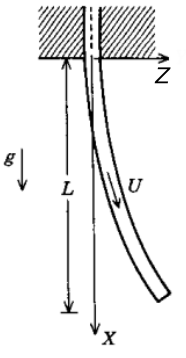
\includegraphics[width=0.15\linewidth]{cantilevered-pipe-schematic}
	\caption{Schematic of a cantilevered pipe conveying fluid}
	\label{fig:cantilevered-pipe-schematic}
\end{figure}


\chapter{Hamilton's principle for equation of motion for a cantilevered pipe conveying fluid}\label{chap:2}

\section{Assumptions}
The fundamental assumptions made for the cantilevered pipe and the fluid are 
\begin{enumerate}[label=(\alph*)]
	\item the fluid is incompressible 
	\item the velocity profile of the fluid is uniform 
	\item the diameter of the pipe is small compared to its length, such that the pipe behaves like an Euler-Bernoulli beam
	\item the motion is planar (2D)
	\item the deflections of the pipe are small
	%\item the deflections of the pipe are large, but the strains are small % for non-linear
	\item rotatory inertia and shear inertia and shear deformation are neglected
	\item the pipe centerline is inextensible 
\end{enumerate}

\section{Geometric details}
Consider the slender cantilevered pipe in its initial undeformed state with its centerline along $X$ axis (see fig \ref{fig:cantilevered-pipe-schematic}). We use two coordinate systems to define the system 
\begin{itemize}
	\item Eulerian: $(x,z)$
	\item Lagrangian: $(x_0, z_0)$
\end{itemize}
For the planar motions in $(x,z)$ plane, the displacements are defined as $u = x - x_0$ and $w = z - z_0 = z$.

\begin{figure}
	\centering
	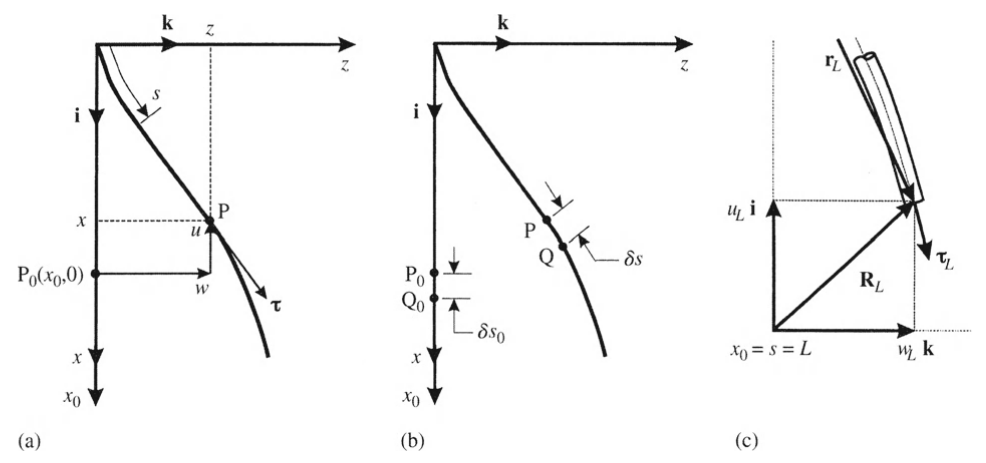
\includegraphics[width=0.8\linewidth]{coordinate-system-pipe}
	\caption{(a) Eulerian ($x,z$) and Lagrangian $(x_0, z_0)$ coordinate systems and the coordinate $s$ when the centerline is taken to be inextensible, (b) for derivation of inextensibility condition, (c) diagram defining terms for the statement of Hamilton's principle}
	\label{fig:coordinate-system-pipe}
\end{figure}

\paragraph{Inextensibility condition}:
Let us consider two points $P$ and $Q$ of the deflected pipe, originally $P_o$ and $Q_o$. We have
\begin{align*}
 (\delta s)^2 = (\delta x)^2 + (\delta z)^2, \qquad (\delta s_0)^2 = (\delta x_0)^2 + (\delta z_0)^2 = (\delta x_0)^2
\end{align*}
Subtracting the second expression from the first,
\begin{align*}
(\delta s)^2 -  (\delta s_0)^2 &= (\delta x)^2 + (\delta z)^2 - (\delta x_0)^2 \\
                     &= \left[\left(\pdv{x}{x_0}\right)^2 + \left(\pdv{z}{x_0}\right)^2 - 1\right](\delta x_0)^2 
\end{align*} 
As $\delta s = \delta s_0 \equiv \delta x_0$, we have the inextensibility condition as
\begin{align}
   \left(\pdv{x}{x_0}\right)^2 + \left(\pdv{z}{x_0}\right)^2 &= 1 \notag \\
 \text{ or, } ~ \left(1 + \pdv{u}{x_0}\right)^2 + \left(\pdv{w}{x_0}\right)^2 &= 1  \label{eqn:inextensibility}
\end{align}
%{\color{red} Order of magnitude analysis}
In order to make approximations for some expressions later on, we assume that the lateral displacement $w$ is small compared to the pipe length $L$, that is,
$$\frac{w}{L} \sim \mathcal{O} (\epsilon), ~\quad \epsilon << 1$$
Using inextensibility condition, binomial approximation and replacing $x_0$ by $s$, we can deduce 
\begin{align*}
   u \simeq - \int_0^s \frac{1}{2} \bigg(\pdv{w}{s}\bigg)^2~ds, \quad \frac{u}{L} \sim \mathcal{O} (\epsilon^2)
\end{align*}

%%%%%%%%%%% HAMILTONIAN DERIVATION
\section{Hamiltonian derivation}
We begin with the principle of virtual work for a system of $N$ particles with individual mass $m_i$ subjected to a force $\vb*{F}_i$. From d'Alembert's principle
\begin{align}
   \sum_{i=1}^N (m_i\ddot{\vb*{r}}_i - \vb*{F}_i)\cdot \delta \vb*{r}_i = 0 \label{eqn:dAlembert}
\end{align}
with $\vb*{r}_i$ being the position vector of each particle and $\delta \vb*{r}_i$ the associated virtual displacement satisfying the system constraints (boundary conditions).

Now, consider the second term of equation \ref{eqn:dAlembert}
\begin{align*}
  \sum_{i=1}^N \vb*{F}_i \cdot \delta \vb*{r}_i = \delta W_{nc} + \delta W_c 
\end{align*}
where $\delta W_{nc}$ is the virtual work due to non-conservative forces while $\delta W_c$ is that due to conservative forces. Taking $\delta W_{nc} =  \delta W$ and $\delta W_c = -\delta V$ ($V$ is the potential energy), we have 
\begin{align*}
\sum_{i=1}^N \vb*{F}_i \cdot \delta \vb*{r}_i = \delta W - \delta V 
\end{align*}
Going back to the first term on eqn \ref{eqn:dAlembert}, 
\begin{align}
\sum_{i=1}^N m_i\ddot{\vb*{r}}_i \cdot \delta \vb*{r}_i &= \sum_{i=1}^N m_i\dv{(\dot{\vb*{r}}_i \cdot \delta \vb*{r}_i)}{t}  - \sum_{i=1}^N \frac{1}{2} m_i\delta (\dot{\vb*{r}}_i \cdot \dot{\vb*{r}_i}) \\
  &= \sum_{i=1}^N m_i\dv{(\dot{\vb*{r}}_i \cdot \delta \vb*{r}_i)}{t}  - \delta \underbrace{\sum_{i=1}^N \frac{1}{2} m_i (\dot{\vb*{r}}_i \cdot \dot{\vb*{r}_i})}_{T} \\
  &= \sum_{i=1}^N m_i \dv{(\dot{\vb*{r}}_i \cdot \delta \vb*{r}_i)}{t} - \delta T
\end{align}
with $T$ being the kinetic energy of the system \\
Substituting the expressions for the corresponding terms in eqn \ref{eqn:dAlembert} gives
\begin{align*}
\sum_{i=1}^N m_i\dv{(\dot{\vb*{r}}_i \cdot \delta \vb*{r}_i)}{t} - \delta T - (\delta W - \delta V ) = 0 \\
\implies~ \delta (T - V) + \delta W - \sum_{i=1}^N m_i \dv{(\dot{\vb*{r}}_i \cdot \delta \vb*{r}_i)}{t} = 0
\end{align*}
Let us have the Lagrangian function, $\mathcal{L} = T - V$, such that the above equation becomes
\begin{align}
\delta \mathcal{L} + \delta W - \sum_{i=1}^N m_i \dv{(\dot{\vb*{r}}_i \cdot \delta \vb*{r}_i)}{t} = 0 \notag \\
\implies~ \delta \mathcal{L} + \delta W - \dv{}{t}\sum_{i=1}^N \bigg(m_i\dot{\vb*{r}}_i \cdot \delta \vb*{r}_i\bigg) = 0 \label{eqn:virtual-work-eqn}
\end{align}
Let us extend this idea to a continuous, closed system associated with a control volume $\mathcal{V}_c (t)$ bounded by a surface $\mathcal{S}_c (t)$, composed of particles of density $\rho$, each with position vector $\vb*{r}$ and velocity $\vb*{u}$. Applying the principle of virtual work, eqn \ref{eqn:virtual-work-eqn}
\begin{align}
   \delta \mathcal{L}_c + \delta W - \frac{D}{Dt}\int_{\mathcal{V}_c(t)} \rho (\vb*{u}\cdot \delta \vb*{r})d\mathcal{V} = 0 \label{eqn:virtual-work-closed-system}
\end{align}
where $\mathcal{L}_c = T_c - V_c$ is the Lagrangian function of the closed system, $\delta W$ is the virtual work due to generalized forces and $\frac{D}{Dt}$ is the material derivative along a particle; hence, $\vb*{u} = \frac{D\vb*{r}}{Dt}$. \\
Hamilton's principle can be obtained by integrating the equation \ref{eqn:virtual-work-closed-system} between two instants, $t_1$ and $t_2$.
  \begin{align*}
   \int_{t_1}^{t_2} \left[\delta \mathcal{L}_c + \delta W - \frac{D}{Dt}\int_{\mathcal{V}_c(t)} \rho (\vb*{u}\cdot \delta \vb*{r})d\mathcal{V}\right] dt = 0 \\
   \int_{t_1}^{t_2}\delta \mathcal{L}_cdt + \int_{t_1}^{t_2} \delta W~dt - \int_{t_1}^{t_2}\frac{D}{Dt}\int_{\mathcal{V}_c(t)} \rho (\vb*{u}\cdot \delta \vb*{r})d\mathcal{V}~ dt = 0
  \end{align*}
Noting that $\vb*{r}$ is prescribed at $t_1$ and $t_2$, that is $\delta\vb*{r} = \vb*{0}$ resulting in 
 \begin{align*}
\int_{t_1}^{t_2}\delta \mathcal{L}_cdt + \int_{t_1}^{t_2} \delta W~dt = 0 \\
\delta \int_{t_1}^{t_2}\mathcal{L}_cdt + \delta \int_{t_1}^{t_2}W~dt = 0 
\end{align*}

Extending it to an open system is done by considering a portion $\mathcal{S}_o (t)$ of the surface of the control volume $\mathcal{V}_o (t)$ to have a velocity $\vb*{V}\cdot \vb*{n}$ normal to the surface ($\vb*{n}$ is the surface normal), across which mass may be transported. Portion $\mathcal{S}_c (t)$ corresponds to the closed part. Fig \ref{fig:open-and-closed-portions} shows the system at time $t$ and time $t+dt$. On the closed portion $\mathcal{S}_c (t)$, $\vb*{V}\cdot \vb*{n} = \vb*{u}\cdot \vb*{n}$.
%The open system does not necessarily hac have the same particles

Should, at time $t$, $\mathcal{V}_o (t)$, coincides with $\mathcal{V}_c (t)$ as shown in fig \ref{fig:open-and-closed-portions} (a), then Reynolds' general transport theorem states that the total rate of change in $\{ ~\}$ is equal to the rate of change in the volume and that due to influx/efflux through the boundaries, that is
\begin{align}
  \dv{}{t} \int_{\mathcal{V}_o (t)} \{~\}d\mathcal{V} = \frac{D}{Dt} \int_{\mathcal{V}_c (t)} \{~ \} d\mathcal{V} + \int_{\mathcal{S}_o} \{ ~\} (\vb*{V} - \vb*{u}) \cdot \vb*{n} d\mathcal{S} \label{eqn:reynolds-transport-theorem}
\end{align}
where 
\begin{align*}
  \frac{D}{Dt} \int_{\mathcal{V}_c (t)} \{~ \} d\mathcal{V} = \frac{D}{Dt} \int_{\mathcal{V}_o (t)} \{~ \} d\mathcal{V}
\end{align*}

\begin{figure}[h!]
	\centering
	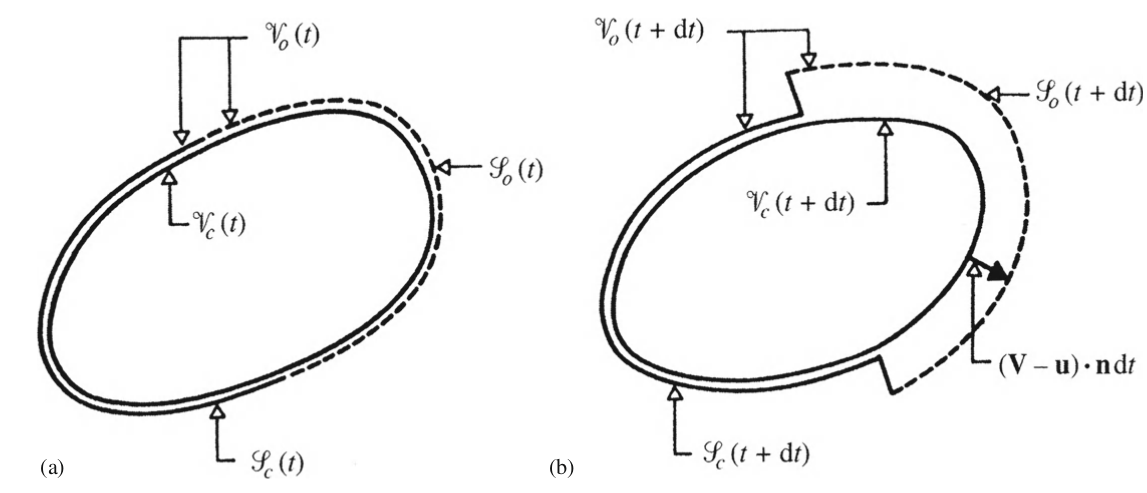
\includegraphics[width=0.8\textwidth]{open-and-closed-portions}
	\caption{Control volume of the open system under consideration, $\mathcal{V}_o$, and a fictitious closed system $\mathcal{V}_c$, coincident with $\mathcal{V}_o$ at time $t$. Control surfaces $\mathcal{S}_o$ and $\mathcal{S}_c$ are associated with the open and closed parts of the open system. (a) System at time $t$, (b) at time $t + dt$}
	\label{fig:open-and-closed-portions}
\end{figure}

Subtituting \ref{eqn:reynolds-transport-theorem} and the above relation into \ref{eqn:virtual-work-closed-system} gives
\begin{align*}
 \delta \mathcal{L}_o + \delta W + \int_{\mathcal{S}_o} \rho (\vb*{u}\cdot \delta \vb*{r}) (\vb*{V} - \vb*{u}) \cdot \vb*{n} d\mathcal{S} -
 \dv{}{t} \int_{\mathcal{V}_o (t)} \rho (\vb*{u}\cdot \delta \vb*{r})d\mathcal{V} = 0
\end{align*}
where $\mathcal{L}_o$ is the Lagrangian of the open system.


Upon integrating with respect to time from $t_1$ to $t_2$ and using $\delta \vb*{r} = \vb*{0}$ at the integration limits, we obtain the Hamilton's principle for the open system
\begin{align}
  \delta \int_{t_1}^{t_2}\mathcal{L}_o~dt + \delta \int_{t_1}^{t_2} W~dt + \int_{t_1}^{t_2}\left[\int_{\mathcal{S}_o} \rho (\vb*{u}\cdot \delta \vb*{r}) (\vb*{V} - \vb*{u}) \cdot \vb*{n} d\mathcal{S}\right] dt - \int_{t_1}^{t_2} \left[
 \dv{}{t} \int_{\mathcal{V}_o (t)} \rho (\vb*{u}\cdot \delta \vb*{r})d\mathcal{V}\right] dt &= 0 \notag \\
 \implies~\delta \int_{t_1}^{t_2}\mathcal{L}_o~dt + \int_{t_1}^{t_2} \underbrace{\left[\delta W + \int_{\mathcal{S}_o}\rho (\vb*{u}\cdot \delta \vb*{r}) (\vb*{V} - \vb*{u}) \cdot \vb*{n} d\mathcal{S}\right]}_{\delta H} dt & = 0 \notag \\
 \implies~\delta \int_{t_1}^{t_2}\mathcal{L}_o~dt + \delta \int_{t_1}^{t_2}  H dt &= 0  \label{eqn:L-H}
\end{align}

Let us now apply the above equation to a cantilevered pipe conveying a fluid. For the sake of simplicity, we consider the case of no dissipation and  a constant flow velocity $U$. Also it is assumed that the only force involved in $\delta W$ is due to the pressure $p$, measured above the ambient of the surrounding medium, ($p$ is gauge pressure) and hence
\begin{align*}
   \delta W &= - \int_{\mathcal{S}_c(t) + \mathcal{S}_i + \mathcal{S}_e(t)} p (\delta \vb*{r} \cdot \vb*{n}) d\mathcal{S} \\
   \delta H &= - \int_{\mathcal{S}_c(t) + \mathcal{S}_i + \mathcal{S}_e(t)} p (\delta \vb*{r} \cdot \vb*{n}) d\mathcal{S} + \int_{\mathcal{S}_i + \mathcal{S}_e(t)}\rho (\vb*{u}\cdot \delta \vb*{r}) (\vb*{V} - \vb*{u}) \cdot \vb*{n} d\mathcal{S}
\end{align*}
where $\mathcal{S}_c(t)$ is the surface covered by the pipe wall, and $\mathcal{S}_i$ (note that $\mathcal{S}_i$ is not dependent on $t$) and $\mathcal{S}_e(t)$ are the inlet and exit open surfaces for the fluid. 

It is presumed that any virtual displacement of the pipe does not induce a virtual displacement of the fluid relative to the pipe. And so, virtual displacements of the fluid relative to the pipe are independent of those of the pipe. As the fluid is incompressible too, there can be no virtual change in the volume of the system and so, the integral over $\mathcal{S}_c(t)$ can be dropped and the above relation becomes
\begin{align*}
\delta H = - \int_{\mathcal{S}_i + \mathcal{S}_e(t)} p (\delta \vb*{r} \cdot \vb*{n}) d\mathcal{S} + \int_{\mathcal{S}_i + \mathcal{S}_e(t)}\rho (\vb*{u}\cdot \delta \vb*{r}) (\vb*{V} - \vb*{u}) \cdot \vb*{n} d\mathcal{S}
\end{align*}
 If the fluid entrance conditions are prescribed and are constant, then the integrals over $\mathcal{S}_i$ are zero. Also, since $p=0$ at the outlet, the first term vanishes for the above equation
\begin{align*}
\delta H = \int_{\mathcal{S}_e(t)}\rho (\vb*{u}\cdot \delta \vb*{r}) (\vb*{V} - \vb*{u}) \cdot \vb*{n} d\mathcal{S}
\end{align*} 
It would be shown in chapter \ref{chap:3} that $\vb*{u} = \dot{\vb*{r}} + U\vb*{\tau}$ where $\vb*{r} = x\vb*{i} + z\vb*{k}$, $\vb*{\tau} = \pdv{x}{s}\vb*{i} + \pdv{z}{s} \vb*{k}$ and $(\dot{})$ indicates differentiation with respect to $t$. Also, using $(\vb*{u} - \vb*{V})\cdot \vb*{n} = U$ at $\mathcal{S}_e (t)$ and $M = \rho A$ ($A$ being the area of the outlet), we have
\begin{align*}
\delta H = - MU (\dot{\vb*{r}}_L + U\vb*{\tau}_L)\cdot \delta\vb*{r}_L 
\end{align*}
Substituting the above relation in eqn \ref{eqn:L-H}, we have 
\begin{align}
\delta \int_{t_1}^{t_2}\mathcal{L}_o~dt - \int_{t_1}^{t_2}  MU (\dot{\vb*{r}}_L + U\vb*{\tau}_L)\cdot \delta\vb*{r}_L  dt = 0 \label{eqn:Lo}
\end{align}
where $\vb*{r}_L$ and $\vb*{\tau}_L$ are the position vector and the tangential unit vector at the end of the pipe as seen in fig \ref{fig:coordinate-system-pipe} (c).

%%%%%%%%%%% started derivation of linear equation
\chapter{Linear governing equation for small transverse displacement}\label{chap:3}

%%%%%%%%%%%%%%%%%%%%%
\section{Derivation of the equation of motion}
From eqn \ref{eqn:Lo}, we have the following
\begin{align*}
\delta \int_{t_1}^{t_2}\mathcal{L}_o~dt -  \int_{t_1}^{t_2}  MU (\dot{\vb*{r}}_L + U\vb*{\tau}_L)\cdot \delta\vb*{r}_L  dt = 0
\end{align*}
Let us redefine the Lagrangian of the system, $\mathcal{L}$ (drop the subscript $o$) in eqn \ref{eqn:Lo} as
\begin{align}
\mathcal{L} = T- V \label{eqn:Lo1}
\end{align}
where $T$ is the total kinetic energy  and $V$ is the total potential energy of the system. 

\subsubsection{Certain useful relationships}\label{subsec:relationships}
Before we start building expressions for the different terms of eqn \ref{eqn:Lo1}, we derive the following useful relationships

\begin{itemize}
\item $u = x - x_o \implies u = x - s ~~(\text{as } x_o = s)$. 
 Upon differentiating with respect to $t$, we have
   $$\dot{x} = \dot{u}$$
 
 \item From inextensibility condition (eqn \ref{eqn:inextensibility}), we have
     \begin{align*}
        \left(\pdv{x}{s}\right)^2 + \left(\pdv{z}{s}\right)^2 &= 1\\
    \implies ~~ \pdv{x}{s} &= \sqrt{1 - \left(\pdv{w}{s}\right)^2} \quad (\text{as } z = w) \\
           &\approx 1 - \frac{1}{2}\left(\pdv{w}{s}\right)^2 \quad \left(\text{considering } \frac{w}{L}\sim O(\epsilon)\right)\\
           &= 1 - \frac{1}{2}w'^2 \\
      \implies ~~ \pdv{u}{s} + \underbrace{\pdv{s}{s}}_{1} &= 1 - \frac{1}{2}w'^2  \\
      \implies~~ \pdv{u}{s} &=  - \frac{1}{2}w'^2
     \end{align*}
     Upon integrating with respect to $s$ and using the boundary condition $u(s=0) = 0$
     \begin{align*}
        u(s) = - \frac{1}{2} \int_0^s w'^2 ~ds
     \end{align*}
    \item $\dot{\vb*{r}}_L = \dot{x}_L \vb*{i} + \dot{z}_L \vb*{k} = \dot{u}_L \vb*{i} + \dot{w}_L \vb*{k} $
    
    \item $\vb*{\tau}_L = x_L' \vb*{i} + z_L'\vb*{k} \approx \left(1 - \frac{1}{2}\int_0^L w'^2~ds\right) \vb*{i} + w_L' \vb*{k}$, where prime ($'$) indicates differentiation with respect to $s$.
    \item $\delta \vb*{r}_L = \delta u_L \vb*{i} + \delta w_L \vb*{k}$
\end{itemize}
Using the relationships derived above in the second term of eqn \ref{eqn:Lo1} 
\begin{align*}
 & \int_{t_1}^{t_2}  MU (\dot{\vb*{r}}_L + U\vb*{\tau}_L)\cdot \delta\vb*{r}_L  dt \\
 =& \int_{t_1}^{t_2} MU \left[\dot{u}_L \vb*{i} + \dot{w}_L \vb*{k} + U\left(1 - \frac{1}{2}\int_0^L w'^2~ds\right) \vb*{i} + Uw_L' \vb*{k}\right]\cdot (\delta u_L \vb*{i} + \delta w_L \vb*{k})~dt \\
 =&\int_{t_1}^{t_2} MU \left[\left(\dot{u}_L + U\left(1 - \frac{1}{2}\int_0^L w'^2~ds\right)\right)\delta u_L + \left(\dot{w}_L + Uw_L'\right)\delta w_L\right]~dt \\
 =& \int_{t_1}^{t_2}MU\left[ \underbrace{\dot{u}_L\delta u_L}_{\text{neglecting}} + \underbrace{U\left(1 - \frac{1}{2}\int_0^L w'^2~ds\right)}_{\approx ~U}\delta u_L + \left(\dot{w}_L + Uw_L'\right)\delta w_L\right]~dt \\
  \approx&  \int_{t_1}^{t_2}\left[ MU^2\delta u_L + MU\left(\dot{w}_L + Uw_L'\right)\delta w_L\right]~dt
\end{align*}
Substituting this in eqn \ref{eqn:Lo1} and rearranging, we get
\begin{align}
\delta \int_{t_1}^{t_2}\mathcal{L}~dt - \int_{t_1}^{t_2}\left[ MU^2\delta u_L + MU\left(\dot{w}_L + Uw_L'\right)\delta w_L\right]~dt &= 0 \notag \\
\implies~~\delta \int_{t_1}^{t_2} (\mathcal{L} - MU^2 u_L)~dt - \int_{t_1}^{t_2}MU\left(\dot{w}_L + Uw_L'\right)\delta w_L~dt &= 0 \label{eqn:Lo2}
\end{align}

\subsection{Kinetic energy of the system} 
The total kinetic energy of the system is 
\begin{align}
T = T_p + T_f
\end{align}
where $T_p$ and $T_f$ are the kinetic energies associated with the pipe and the enclosed fluid.

Let us consider a small segment of pipe and fluid (see fig \ref{fig:coordinate-system-pipe}). By definition, velocity of the pipe element is
\begin{align*}
\vb*{V}_p = \pdv{\vb*{r}}{t} = \dot{x}\vb*{i} + \dot{z}\vb*{k}
\end{align*}
Velocity of the fluid element is 
\begin{align*}
\vb*{V}_f = \vb*{V}_p + U \vb*{\tau}
\end{align*}
where $\vb*{\tau}$ is the tangential unit vector, $\vb*{\tau} = x' \vb*{i} + z'\vb*{k}$. And so, 
\begin{align*}
\vb*{V}_f = \dot{x}\vb*{i} + \dot{z}\vb*{k} + U\left(x' \vb*{i} + z'\vb*{k}\right) = (\dot{x} + Ux')\vb*{i} + (\dot{z} + Uz')\vb*{k})
\end{align*}
Kinetic energy of the pipe, 
$$T_p = \frac{1}{2}m \int_0^L \vb*{V}_p\cdot\vb*{V}_p~ds =  \frac{1}{2}m \int_0^L (\dot{x}^2 + \dot{z}^2) ds$$
where $m$ is the linear mass density of the pipe \\
Kinetic energy of the fluid, 
\begin{align*}
   T_f &=  \frac{1}{2}M \int_0^L \vb*{V}_f\cdot\vb*{V}_f~ds  \\
      & = \frac{1}{2}M \int_0^L \left[ (\dot{x} + Ux')^2 + (\dot{z} + Uz')^2\right] ds  \\
      &= \frac{1}{2}M \int_0^L \left(\dot{x}^2 + 2U\dot{x}x' + U^2x'^2 + \dot{z}^2 + 2U\dot{z}z' + U^2z'^2\right) ds \\
      &= \frac{1}{2}M \int_0^L \left(\dot{x}^2 + 2U\dot{x}x' + U^2\underbrace{(x'^2 + z'^2)}_{= 1 \text{ using } \ref{eqn:inextensibility}} \dot{z}^2 + 2U\dot{z}z'\right) ds
\end{align*}
where $M$ is the linear mass density of the fluid. \\
Let us make some approximations
\begin{align*}
  \dot{x} &\sim O(\epsilon^2) \\
   x' &\approx 1  - \frac{1}{2}w'^2 \approx 1
\end{align*}
Also as $\dot{x} = \dot{u}$ and $z = w$,
\begin{align*}
T_p = \frac{1}{2}m \int_0^L \dot{w}^2~ds, \qquad T_f = \frac{1}{2}M\int_0^L \left(U^2 + \dot{w}^2 + 2U\dot{w}w' + 2U\dot{w}w' + 2U\dot{u}\right)~ds 
\end{align*}
therefore, 
\begin{align}
T = \frac{1}{2}m \int_0^L \dot{w}^2~ds + \frac{1}{2}M\int_0^L \left(U^2 + \dot{w}^2 + 2U\dot{w}w' + 2U\dot{w}w' + 2U\dot{u}\right)~ds \label{eqn:T}
\end{align}

\subsection{Potential energy of the system} 
The total potential energy of the system comprises of gravitational energy and strain energy stored in the pipe, and the gravitational energy stored in the fluid, that is
$$V = V_p + V_f$$
In general, gravitational energy of a mass of density $\rho$ immersed in a uniform gravitational field of strength $g$ is given by $G = -\int_\mathcal{V} \rho\vb*{g} \cdot \vb*{\xi}d\mathcal{V}$, where $\vb*{\xi}$ is the position vector of a mass element with respect to some origin. \\
Potential energy of the pipe is 
$$V_p =   \frac{1}{2} EI \int_0^L  w''^2 ds - mg\int_0^L u ~ds$$
where $E$ is the Young's modulus and $I$ is the area moment of inertia. \\
Substituting $u(s) = -\frac{1}{2} \int_0^s w'^2 ~ds$ in the above \\
$$V_p =   \frac{1}{2} EI \int_0^L  w''^2 ds + \frac{1}{2}mg\int_0^L \left(\int_0^s w'^2 ~ds\right)~ds$$
Similarly, the potential energy of the fluid is
$$V_f  = \frac{1}{2}Mg\int_0^L \left(\int_0^s w'^2 ~ds\right)~ds$$
Now, 
$$V = \frac{1}{2} EI \int_0^L  w''^2 ~ds + \frac{1}{2}(m + M)g\int_0^L \left(\int_0^s w'^2 ~ds\right)~ds$$
Let us simplify the second term using integration by parts
\begin{align*}
\frac{1}{2}(m + M)g\int_0^L 1\cdot \left(\int_0^s w'^2 ~ds\right)~ds &= \frac{1}{2}(m + M)g \left[s\int_0^s w'^2 ~ds\bigg|_0^L - \int_0^L s w'^2 ~ds \right]  \\
&= \frac{1}{2}(m + M)g\left[L\int_0^L w'^2 ~ds - \int_0^L s w'^2 ~ds \right] \\
&= \frac{1}{2}(m + M)g\int_0^L (L - s) w'^2 ~ds
\end{align*}
The total potential energy of the system is
\begin{align}
V = \frac{1}{2} EI \int_0^L  w''^2 ds + \frac{1}{2}(m + M)g\int_0^L (L - s) w'^2 ~ds \label{eqn:V}
\end{align}

\subsection{Expanding variational terms}
Expanding the term $\delta \int_{t_1}^{t_2} (\mathcal{L} - MU^2\delta u_L)~dt$ of eqn \ref{eqn:Lo2}, we have
\begin{align*}
  \delta \int_{t_1}^{t_2} (\mathcal{L} - MU^2\delta u_L)~dt &= \delta \int_{t_1}^{t_2} (T - V - MU^2\delta u_L)~dt \\
  &= \delta \int_{t_1}^{t_2} T~dt  - \delta \int_{t_1}^{t_2} V~dt - \delta \int_{t_1}^{t_2} MU^2\delta u_L~dt
\end{align*}
Using eqn \ref{eqn:T}, we have
\begin{align*}
 \delta \int_{t_1}^{t_2} T~dt &= \int_{t_1}^{t_2} \left[m \int_0^L \dot{w}\delta \dot{w}~ds + M\int_0^L \left(\dot{w}\delta \dot{w} + U\dot{w}\delta w' + U w'\delta \dot{w} + U\delta \dot{u}\right)~ds \right]~dt \\
  &=   \int_0^L (m + M)\left(\int_{t_1}^{t_2} \dot{w}\delta \dot{w}~dt\right)~ds + \int_{t_1}^{t_2} MU\bigg(\int_0^L \dot{w}\delta w'~ds\bigg)~dt \\
  &\phantom{=} + \int_0^L MU\bigg(\int_{t_1}^{t_2} w'\delta \dot{w}~dt\bigg)~ds  + \int_0^L MU\bigg(\int_{t_1}^{t_2}\delta \dot{u}~dt\bigg)~ds  \\
  &= \int_0^L (m + M) \left(\dot{w}\delta w\bigg|_{t_1}^{t_2} - \int_{t_1}^{t_2} \ddot{w}\delta w~dt\right)~ds + \int_{t_1}^{t_2} MU\bigg(\dot{w}\delta w\bigg|_0^L - \int_0^L \dot{w}'\delta w~ds\bigg)~dt  \\
  &\phantom{=} + \int_0^L MU\bigg(w'\delta w\bigg|_{t_1}^{t_2} - \int_{t_1}^{t_2} \dot{w}'\delta w~dt\bigg)~ds + \int_0^L MU\bigg(\delta u\bigg|_{t_1}^{t_2}\bigg)~ds 
\end{align*}
From the Hamilton's principle that the variations at $t=t_1$ and $t=t_2$ are zero, we have $\delta w|_{t_1} = \delta w_{t_2} = \delta u|_{t_1} = \delta u|_{t_2} = 0$. Using BCs, we have $\delta w|_{s = 0} = 0$ (clamped at $s=0$). So,
\begin{align}
\delta \int_{t_1}^{t_2} T~dt &= -\int_0^L\int_{t_1}^{t_2} (m + M) \ddot{w}\delta w~dt~ds - \int_{t_1}^{t_2}\int_0^L 2MU\dot{w}'\delta w~ds~dt  + \int_{t_1}^{t_2} MU\dot{w}_L\delta w_L~dt  \label{eqn:variation-in-T}
\end{align}
Using equation \ref{eqn:V}, we have
\begin{align*}
 \delta \int_{t_1}^{t_2} V~dt &= \delta \int_{t_1}^{t_2} \bigg[\frac{1}{2} EI \int_0^L  w''^2 ds + \frac{1}{2}(m + M)g\int_0^L (L - s) w'^2 ~ds \bigg]~dt \\
    &=\int_{t_1}^{t_2} \bigg[EI \int_0^L  w''\delta w'' ds + (m + M)g\int_0^L (L - s) w'\delta w'~ds \bigg]~dt \\
    &=\int_{t_1}^{t_2} EI \bigg[w''\delta w'\bigg|_0^L - \int_0^L  w'''\delta w' ds\bigg]~dt \\
    &\phantom{=}~~ + \int_{t_1}^{t_2}(m + M)g\bigg[(L - s) w'\delta w\bigg|_0^L - \int_0^L ((L - s) w')'\delta w~ds \bigg]~dt  \\
    &=\int_{t_1}^{t_2} EI \bigg[w''\delta w'\bigg|_0^L - w'''\delta w\bigg|_0^L +  \int_0^L  w''''\delta w ds\bigg]~dt \\
    &\phantom{=}~~ + \int_{t_1}^{t_2}(m + M)g\bigg[(L - s) w'\delta w\bigg|_0^L - \int_0^L ((L - s) w')'\delta w~ds \bigg]~dt
\end{align*}
Using the following BCs
$$w(s=0) = w'(s=0) = 0; ~ w''(s=L) = w'''(s=L)= 0$$
We now have
\begin{align}
  \delta \int_{t_1}^{t_2} V~dt &= \int_{t_1}^{t_2}\int_0^L  EI w''''\delta w ds~dt - \int_{t_1}^{t_2}\int_0^L (m + M)g ((L - s) w')'\delta w~ds~dt \label{eqn:variation-in-V}
\end{align}
Expanding the second term in the first integral on the left of eqn \ref{eqn:Lo2} using the certain useful relations, we have
\begin{align*}
\delta \int_{t_1}^{t_2}MU^2 u_L~dt &= \delta \int_{t_1}^{t_2}MU^2\left(-\frac{1}{2}\int_0^L w'^2~ds\right)~dt \\
    &= -\int_{t_1}^{t_2}MU^2\left(\int_0^L w'\delta w'~ds\right)~dt \\
    &= -\int_{t_1}^{t_2}MU^2\left(w'\delta w\bigg|_0^L - \int_0^L w''\delta w~ds\right)~dt \\
\end{align*}
Using the BC $w(s=0) = 0$, we get
\begin{align}
  \delta \int_{t_1}^{t_2}MU^2 u_L~dt &= -\int_{t_1}^{t_2}MU^2w_L'\delta w_L~dt + \int_{t_1}^{t_2}MU^2\int_0^L w''\delta w~ds~dt  \label{eqn:variation-in-MU}
\end{align}
Substituting the expressions \ref{eqn:variation-in-T}, \ref{eqn:variation-in-V} and \ref{eqn:variation-in-MU} in eqn \ref{eqn:Lo2}, we have 
\begin{multline*}
   -\int_0^L\int_{t_1}^{t_2} (m + M) \ddot{w}\delta w~dt~ds - \int_{t_1}^{t_2}\int_0^L 2MU\dot{w}'\delta w~ds~dt  + \cancel{\int_{t_1}^{t_2} MU\dot{w}_L\delta w_L~dt} \\
   - \int_{t_1}^{t_2}\int_0^L  EI w''''\delta w ds~dt + \int_{t_1}^{t_2}\int_0^L (m + M)g ((L - s) w')'\delta w~ds~dt + \cancel{\int_{t_1}^{t_2}MU^2w_L'\delta w_L~dt} \\
    - \int_{t_1}^{t_2}MU^2\int_0^L w''\delta w~ds~dt - \cancel{\int_{t_1}^{t_2}MU\left(\dot{w}_L + Uw_L'\right)\delta w_L~dt} = 0 
\end{multline*}
Thus,
\begin{multline*}
-\int_{t_1}^{t_2} \int_0^L \bigg[(m + M) \ddot{w}\delta w + 2MU\dot{w}' + EI w'''' - (m + M)g ((L - s) w')' + MU^2 w''\bigg]\delta w~ds~dt = 0 
\end{multline*}

\subsection{Equation of motion}
For arbitrary variations in $\delta w$ and using $s \approx x$, we obtain the equation of motion for the cantilevered pipe conveying fluid
\begin{align}
(m + M) \ddot{w} + 2MU \dot{w}' + EI w'''' - (m + M)g\left((L - x)w'\right)' + MU^2w'' &= 0 \notag \\
\implies ~~(m + M) \ddot{w} + 2MU \dot{w}' + EI w''''  + (MU^2- (m + M)g(L - x))w'' + (m + M)gw' &= 0  \label{eqn:linear-cantilevered-pipe}
\end{align}

\subsection{Incorporation of dissipative effects}
In order to complete the equations, we must also incorporate dissipative effects into the system \cite{paidoussis}. Let us assume that the pipe material is viscoelastic and of the Kelvin-Voigt type (strain-rate damping). For this, the strain energy expression is modified as 
\begin{align}
E \rightarrow E\bigg(1 + a\pdv{}{t}\bigg) \label{eqn:linear-dissipation-effect}
\end{align} 
where $a$ is the coefficient of Kelvin-Voigt damping in the material. Hence, in eqn \ref{eqn:V}, $EI$ is replaced by $EI\bigg(1 + a\pdv{}{t}\bigg)$. 

Also, suppose the pipe undergoes damping due to external medium in which it is carrying out its motion, then we have an additional term in the equation
$$c\pdv{w}{t} \text{ or  } c\dot{w}$$
which is the external dissipation term and $c$ is the damping constant.

\begin{mdframed}
The governing equation of the cantilevered pipe with both external and internal damping is \cite{paidoussis1974} 
\begin{multline}
(m + M) \ddot{w} + 2MU \dot{w}' + c\dot{w} +  aEI \dot{w}'''' + EI w'''' + (MU^2- (m + M)g(L - x))w'' \\ + (m + M)gw' = 0  \label{eqn:linear-cantilevered-pipe-dissipation}
\end{multline}
\end{mdframed}

\section{Non-dimensional equation of motion}
Let us now non-dimensionalize the equation \ref{eqn:linear-cantilevered-pipe-dissipation}. Denoting the dimensions of mass, length and time by $\mathcal{M}, \mathcal{L}$ and $\mathcal{T}$ respectively, we construct the following time-scale
$$L^2\sqrt{\frac{m + M}{EI}} \equiv \mathcal{L}^2\sqrt{\frac{\mathcal{M}\mathcal{L}^{-1}}{\mathcal{M}\mathcal{L}^{-1}\mathcal{T}^{-2}\mathcal{L}^4}} \equiv \mathcal{T}$$

We also have the following non-dimensional variables
\begin{itemize}
	\item $\tau = \frac{t}{{L^2}\sqrt{\frac{m + M}{EI}}} \equiv \frac{\mathcal{T}}{\mathcal{T}}$
	
	\item $\xi = \frac{x}{L} \equiv \frac{\mathcal{L}}{\mathcal{L}}$
	\item $\eta = \frac{w}{L} \equiv \frac{\mathcal{L}}{\mathcal{L}}$ 
\end{itemize}
Now, 
$$t = \tau L^2\sqrt{\frac{m + M}{EI}}, ~~ x = \xi L,~~ w = \eta L$$
Substituting the above expressions in the eqn \ref{eqn:linear-cantilevered-pipe-dissipation}, we have 
\begin{align*}
(m + M) \pdv[2]{(\eta L)}{\left(\tau L^2\sqrt{\frac{m + M}{EI}}\right) } + 2MU \pdv[2]{(\eta L)}{\left(\tau L^2\sqrt{\frac{m + M}{EI}}\right)}{(\xi L)} + c\pdv{(\eta L)}{\left(\tau L^2\sqrt{\frac{m + M}{EI}}\right)}  +  aEI \frac{\partial^5 (\eta L)}{\partial\left(\tau L^2\sqrt{\frac{m + M}{EI}}\right)}{\partial (\xi L)^4} & \\
 + EI \pdv[4]{(\eta L)}{(\xi L)} +  (MU^2 - (m + M)g(L - \xi L))\pdv[2]{(\eta L)}{(\xi L)} + (m + M)g \pdv{(\eta L)}{(\xi L)}  &= 0 \\
\implies ~ \frac{EI}{L^3} \ddot{\eta} + \frac{2MU}{L^2\sqrt{\frac{m + M}{EI}}} \dot{\eta}' + \frac{c}{L\sqrt{\frac{m + M}{EI}}}\dot{\eta}  +  \frac{aEI}{L^5}\sqrt{\frac{EI}{m + M}} \dot{\eta}'''' + \frac{EI}{L^3} \eta''''  +  \left(\frac{MU^2}{L} - (m + M)g(1 - \xi)\right)\eta'' &\\ + (m + M)g\eta'  &= 0
\end{align*}
where  dot ($\dot{}$) amd prime (') indicates differentiation with respect to $\tau$ and $\xi$ respectively.

Multiplying throughout by $\frac{L^3}{EI}$, we have
\begin{multline*}
 \ddot{\eta} + \frac{2MU}{L^2}\sqrt{\frac{EI}{m + M}}\frac{L^3}{EI} \dot{\eta}' + \frac{c}{L}\sqrt{\frac{EI}{m + M}}\frac{L^3}{EI}\dot{\eta}  +  \frac{a}{L^2}\sqrt{\frac{EI}{m + M}} \dot{\eta}'''' + \eta''''  \\
 + \left(\frac{MU^2}{L} - (m + M)g(1 - \xi)\right)\frac{L^3}{EI}\eta''  + \frac{(m + M)gL^3}{EI}\eta'  = 0
\end{multline*}
\begin{multline*}
\implies ~~ \ddot{\eta} + 2\sqrt{\frac{M}{m+ M}}\left(\sqrt{\frac{M}{EI}}UL\right) \dot{\eta}' + \left(\frac{cL^2}{\sqrt{EI (m + M)}}\right)\dot{\eta}  +  \left(\frac{a}{L^2}\sqrt{\frac{EI}{m + M}}\right) \dot{\eta}'''' + \eta''''  \\
+ \left[\left(\sqrt{\frac{M}{EI}}UL\right)^2 + \left(\frac{(m + M)gL^3}{EI}\right)(\xi - 1)\right]\eta''  + \left(\frac{(m + M)gL^3}{EI}\right)\eta'  = 0
\end{multline*}
We have the following non-dimensional system parameters
\begin{itemize} 
	\item $\beta = \frac{M}{m + M} \equiv \frac{\mathcal{M}\mathcal{L}^{-1}}{\mathcal{M}\mathcal{L}^{-1}}$
	\item $\mathcal{U} = \bigg(\frac{M}{EI}\bigg)^{1/2}UL \equiv \big(\frac{\mathcal{M}\mathcal{L}^{-1}}{\mathcal{M}\mathcal{L}^{-1}\mathcal{T}^{-2}\mathcal{L}^4}\big)^{1/2} \mathcal{L}\mathcal{T}^{-1}\mathcal{L}$
	\item $\sigma = \frac{cL^2}{\sqrt{EI (m + M)}} \equiv \frac{\mathcal{M}\mathcal{L}^{-1}\mathcal{T}^{-1}\mathcal{L}^{2}}{\sqrt{\mathcal{M}\mathcal{L}^{-1}\mathcal{T}^{-2}\mathcal{L}^4 \mathcal{M}\mathcal{L}^{-1}}}$
	
	\item $\alpha = \bigg(\frac{EI}{m + M}\bigg)^{1/2}\frac{a}{L^2} \equiv \bigg(\frac{\mathcal{M}\mathcal{L}^{-1}\mathcal{T}^{-2}\mathcal{L}^4}{\mathcal{M}\mathcal{L}^{-1}}\bigg)^{1/2}\frac{\mathcal{T}}{\mathcal{L}^2}$ 
	
	\item $\gamma = \frac{m + M}{EI}L^3g \equiv \frac{\mathcal{M}\mathcal{L}^{-1}}{\mathcal{M}\mathcal{L}^{-1}\mathcal{T}^{-2}\mathcal{L}^4}\mathcal{L}^3\mathcal{L}\mathcal{T}^{-2}$
\end{itemize}

\begin{mdframed}
 Thus, we have the following non-dimensionalized governing equation 
 \begin{align}
 \ddot{\eta} + 2\sqrt{\beta}\mathcal{U}\dot{\eta}' + \sigma\dot{\eta}  +  \alpha \dot{\eta}'''' + \eta'''' + \left[\mathcal{U}^2 - \gamma (1 - \xi)\right]\eta''  + \gamma\eta'  = 0 \label{eqn:non-dimensional-linear-cantilevered-pipe-dissipation}
 \end{align}
\end{mdframed}

\section{Transformation into modal equation form}
Let us use Galerkin's method to approximate the solution for eqn \ref{eqn:non-dimensional-linear-cantilevered-pipe-dissipation} \cite{paidoussis1974}. We introduce a solution of the form
\begin{align}
\eta(\xi, \tau) = \sum_{j=1}^N q_j (\tau)\phi_j (\xi)  \label{eqn:modal-decomposition}
\end{align}
where $\phi_j (\xi)$ is the $j^{th}$ modal shape function for the cantilever beam and $q_j (\tau)$ is its corresponding modal coordinate and $N$ is the number of modes considered for approximating the solution.

Substituting the above expression in eqn \ref{eqn:non-dimensional-linear-cantilevered-pipe-dissipation}, multiplying by $\phi_i (\xi)$ and integrating from $\xi = 0$ to $\xi = 1$ on both sides (also invoking Einstein summation notation)

\begin{multline*}
  \int_0^1 \phi_j \ddot{q}_j \phi_i d\xi + 2\sqrt{\beta}\mathcal{U} \int_0^1 \phi_j' \dot{q}_j \phi_i d\xi + \sigma \int_0^1 \phi_j \dot{q}_j \phi_i d\xi  +  \alpha   \int_0^1 \phi_j'''' \dot{q}_j \phi_i d\xi +  \int_0^1 \phi_j'''' q_j \phi_i d\xi \\
   +  \left[\mathcal{U}^2 + \gamma (\xi - 1)\right]\int_0^1 \phi_j'' q_j \phi_i d\xi  + \gamma \int_0^1 \phi_j' q_j \phi_i d\xi  = 0 \qquad i,j = 1,2, \dots, N
\end{multline*}

\begin{multline*}
\implies~~\left(\int_0^1\phi_i \phi_j d\xi\right) \ddot{q}_j+ 2\sqrt{\beta}\mathcal{U} \left(\int_0^1 \phi_i \phi_j' d\xi\right) \dot{q}_j + \sigma \left(\int_0^1 \phi_i\phi_j  d\xi\right)\dot{q}_j +  \alpha  \left( \int_0^1 \phi_i \phi_j''''d\xi\right) \dot{q}_j  +  \left(\int_0^1\phi_i \phi_j''''  d\xi\right)q_j \\
+  \left[\mathcal{U}^2 + \gamma (\xi - 1)\right] \left( \int_0^1 \phi_i\phi_j''   d\xi\right)q_j   + \gamma \left(\int_0^1 \phi_i\phi_j'd\xi\right)q_j = 0 \qquad i,j = 1,2, \dots, N
\end{multline*}
Using the orthonormal property of the modal shapes, that is, $\int_0^1\phi_i \phi_j d\xi = \delta_{ij}$ ($\delta_{ij}$ is the Kronecker delta function), and $\int_0^1\phi_i \phi_j'''' d\xi = \lambda_j^4\delta_{ij}$ where $\lambda_j$ is the $j^{th}$ eigenfrequency
\begin{multline*}
\delta_{ij} \ddot{q}_j+ \left[2\sqrt{\beta}\mathcal{U} \int_0^1 \phi_i \phi_j' d\xi  + \sigma \delta_{ij} +  \alpha  \lambda_j^4\delta_{ij} \right]\dot{q}_j  + \bigg[\lambda_j^4\delta_{ij}  \\
+  \mathcal{U}^2 + \gamma (\xi - 1) \int_0^1 \phi_i\phi_j''   d\xi   + \gamma \int_0^1 \phi_i\phi_j'd\xi\bigg]q_j = 0 \qquad i,j = 1,2, \dots, N
\end{multline*}
Upon rearranging, we get
\begin{multline*}
\delta_{ij} \ddot{q}_j + \left[2\sqrt{\beta}\mathcal{U} \underbrace{\int_0^1 \phi_i \phi_j' d\xi}_{b_{ij}}  + (\sigma +  \alpha  \lambda_j^4) \delta_{ij} \right]\dot{q}_j  + \bigg[\lambda_j^4\delta_{ij} +  (\mathcal{U}^2 - \gamma)\underbrace{\int_0^1 \phi_i\phi_j'' d\xi}_{c_{ij}}  \\ + \gamma \underbrace{\int_0^1 \xi\phi_i\phi_j'' d\xi}_{d_{ij}}  + \gamma \underbrace{\int_0^1 \phi_i\phi_j'd\xi}_{b_{ij}}\bigg]q_j = 0 \qquad i,j = 1,2, \dots, N
\end{multline*}
where
\begin{align*}
   b_{ij} = \int_0^1 \phi_i \phi_j' d\xi \qquad c_{ij} = \int_0^1 \phi_i\phi_j'' d\xi \qquad d_{ij} = \int_0^1 \xi\phi_i\phi_j'' d\xi
\end{align*}
Now,
\begin{multline}
\underbrace{\delta_{ij}}_{M_{ij}} \ddot{q}_j + \underbrace{\left[2\sqrt{\beta}\mathcal{U} b_{ij}  + (\sigma +  \alpha  \lambda_j^4) \delta_{ij} \right]}_{C_{ij}}\dot{q}_j  + \underbrace{\bigg[\lambda_j^4\delta_{ij} +  (\mathcal{U}^2 - \gamma)c_{ij} + \gamma d_{ij}  + \gamma b_{ij}\bigg]}_{K_{ij}}q_j = 0 \qquad i,j = 1,2, \dots, N    \label{eqn:modal-equation}
\end{multline}
where $M_{ij}$, $C_{ij}$ and $K_{ij}$ are the components of mass ($\vb*{M}$), damping ($\vb*{C}$) and stiffness ($\vb*{K}$) matrices respectively. It is to be noted that $\vb*{M} = \vb*{I}$ (an identity matrix).
\begin{align*}
\implies ~~M_{ij} \ddot{q}_j + C_{ij}\dot{q}_j  + K_{ij}q_j = 0 \qquad i,j = 1,2, \dots, N 
\end{align*}
In matrix form, we have
\begin{align}
   \vb*{I} \ddot{\vb*{q}} + \vb*{C} \dot{\vb*{q}} + \vb*{K}\vb*{q} = \vb*{0}   \label{eqn:modal-matrix-equation}
\end{align}
Taking $\vb*{z} = \dot{\vb*{q}}$, the matrix equation can be expressed in terms of two vector equations
\begin{align*}
       \dot{\vb*{q}} &= \vb*{z} \\
       \dot{\vb*{z}} &= -\vb*{K}\vb*{q} -\vb*{C} \vb*{z}
\end{align*}
which can also be represented as
\begin{align*}
 \underbrace{\begin{bmatrix} \dot{\vb*{q}} \\ \dot{\vb*{z}} \end{bmatrix}}_{\dot{\vb*{x}}} &= \underbrace{\begin{bmatrix} \vb*{0} & \vb*{I} \\ -\vb*{K} & -\vb*{C}  \end{bmatrix}}_{\vb*{A}} \underbrace{\begin{bmatrix} \vb*{q}\\ \vb*{z} \end{bmatrix}}_{\vb*{x}}
\end{align*}
Thus we have the following state space equation
\begin{align}
   \dot{\vb*{x}} = \vb*{Ax}   \label{eqn:state-space-equation}
\end{align}
Introducing a solution of the form $\vb*{x}(\tau) = \vb*{x}_0 e^{i\omega \tau}$, where $\omega$ is complex frequency, that is, $\omega = \real (\omega) + i~\imaginary (\omega)$
\begin{align*}
i\omega \vb*{x}_0 e^{i\omega \tau} &= \vb*{A}\vb*{x}_0 e^{i\omega \tau} \\
\implies ~~\left(i\omega \vb*{I} - \vb*{A}\right)\vb*{x}_0 &= \vb*{0}
\end{align*}
For non-trivial solution $\vb*{x}_0 \neq \vb*{0}$, we must have
\begin{align*}
   \det(i\omega \vb*{I} - \vb*{A}) = 0
\end{align*}
which would give us the eigenvalues $\omega$. The real part ($\real (\omega)$) of $\omega$ is the oscillation frequency of the cantilevered pipe system while the imaginary part ($\imaginary (\omega)$) is an indicator of growth or decay of the amplitude of the oscillation. If $\imaginary (\omega) > 0$, the corresponding modal oscillation decays (system is stable) while $\imaginary (\omega) < 0$ indicates that the corresponding modal oscillation amplifies (system becomes unstable). The system is said to undergo flutter when $\imaginary (\omega)$ becomes zero; the corresponding fluid velocity for the given set of parameters $\beta, \gamma, \alpha$ and $\sigma$ is called flutter flow velocity $\mathcal{U}_f$. Physically, flutter is a self-excited oscillation wherein a system develops a steady oscillatory motion of finite amplitude and constant frequency. Mathematically, it is defined as a Hopf bifurcation \cite{paidoussis}.

\subsection{Determining system response}
In order to determine the system response, two initial conditions (ICs) are required: for displacement $\eta (\xi, 0) = \eta_0 (\xi)$ and for velocity $\dot{\eta}~(\xi, 0) = \dot{\eta}_0 (\xi)$. The modal coordinates for displacement $\vb*{q}$ and velocity $\dot{\vb*{q}}$ are obtained by projecting the given ICs on the Galerkin modes and using the orthonormality property of the modal shape functions \cite{meirovitch}
\begin{align*}
   q_j &=  \int_0^1 \eta_0 (\xi) \phi_j (\xi)~d\xi \qquad j = 1, 2, \dots, N  \\
  \dot{q}_j &= \int_0^1 \dot{\eta}_0 (\xi) \phi_j (\xi)~d\xi
\end{align*}




%\section{Solution methodology}

\chapter{Results: Linear analysis of the cantilevered pipe conveying fluid} \label{chap:4}

The linear analysis for the cantilevered pipe conveying fluid system has been performed taking $N = 10$ Galerkin modes to get as accurate an approximation of the system as possible. Let us study the effect of the various parameters $\beta, \gamma, \alpha$ and $\sigma$ on the system's stability and also flutter flow velocity $\mathcal{U}_f$.

\section{Effect of mass ratio $\beta$}
Let us consider a horizontal system with all dissipation effects neglected, such that the system parameters $\alpha = \gamma = \sigma = 0$, and it depends only on $\beta$. The variation of complex frequency $\omega$ with flow velocity $\mathcal{U}$ for different mass ratios are presented in the figures \ref{fig:rootlocusbeta0.2}, \ref{fig:rootlocusbeta0.295} and \ref{fig:rootlocusbeta0.5}. We make the following observations

\begin{itemize}
	\item For small $\mathcal{U}$, all the coupled modes experience damping, that is, $\imaginary (\omega) > 0$ for every mass ratio $\beta = 0.2, 0.295, 0.5$ presented here. At higher $\mathcal{U}$, $\imaginary (\omega)$ of at least one mode begins to decrease and eventually crosses zero to the negative side and so, the system becomes unstable due to flutter. This mechanism of the solution of the system changing its nature is called Hopf bifurcation.
	
	\item For $\beta = 0.2$, $\imaginary (\omega)$ of the second and fourth modes becomes negative as $\mathcal{U}$ crosses $\sim 5.58$ and $\sim 13.2663$ respectively. For $\beta = 0.295$, $\imaginary (\omega)$ of the second mode becomes negative as $\mathcal{U}$ crosses $\sim 7.24$. For $\beta = 0.5$, $\imaginary (\omega)$ of the third mode becomes negative as $\mathcal{U}$ crosses $\sim 9.27$. One thing to note about $\beta = 0.295$ is that the second mode crosses over to the positive imaginary region for $7.24 < \mathcal{U} < 8$ and then re-enters the negative imaginary region. In this process, the system becomes unstable, regains its stability and loses it again; the system dynamics forming the so-called `instability-restabilization-instability' sequence \cite{paidoussis}.
	
	\item \textbf{Mode exchange}: It is to be noted that the second coupled modes for $\beta = 0.2, 0.295$ bend downwards into the negative imaginary axis while the third mode is continuously marching along the positive imaginary axis. However, an opposite facet is observed for $\beta = 0.5$ where its second mode lies in the positive imaginary region while its third mode moves into the negative imaginary axis. This phenomenon of two modes exchanging their nature is called ``mode exchange'' \cite{gregory1966} \cite{paidoussis}.
	
	\item The details regarding the primary coupled flutter mode number for a particular value of mass ratio $\beta$ and its corresponding flutter flow velocity $\mathcal{U}_f$ are tabulated in table \ref{tab:mass-ratio-flutter-velocity}. The primary flutter mode is the second one for $0 < \beta < 0.4$, the third one for $0.4 \leq \beta < 0.55$, the second one for $0.55 \leq \beta \leq 0.6$ and eventually the first mode for $0.6 < \beta < 1$.
\end{itemize}

\begin{table}[h!]
	\centering
\caption{Primary flutter coupled mode and flutter flow velocity
	for various mass ratios} 
\label{tab:mass-ratio-flutter-velocity} 
	\begin{tabular*}{.6\linewidth}{@{\extracolsep{\fill}}|c|c|c|}
		\hline 
		 Mass ratio  & Primary flutter  & Flutter flow velocity \\
		 $\beta$    &  coupled mode   &  $\mathcal{U}_f$ \\
		\hline
		 0.1 & Second & 4.7487  \\
		 0.2 & Second &  5.5779 \\
		  0.295 & Second &  7.2362 \\
		  0.3 & Second &  8.2161 \\
		  0.35 & Second &  8.5176 \\
		  0.4 & Third &  8.7437 \\
		  0.5 & Third & 9.2714 \\
		  0.55 &  Second    & 9.6321 \\
		  0.6 & Second &  9.9497 \\
		  0.65 & First & 10.3846 \\
		  0.7 &  First  &   12.7387   \\
		  0.8 &  First  &   13.4925   \\
		  0.9 & First   &   14.3216   \\
		\hline
	\end{tabular*}
\end{table}



\begin{figure}[h!]
	\centering
	\includegraphics[width=0.8\linewidth]{../rootLocus_beta_0.2_alpha_0.0_gamma_0.0_sigma_0.0}
	\caption{Variation of complex frequency $\omega$ with non-dimensional flow velocity $\mathcal{U}$ for $\beta = 0.2$; the flow velocity where a mode undergoes flutter ($\mathcal{U}_f$) is marked.}
	\label{fig:rootlocusbeta0.2}
\end{figure}

\begin{figure}[h!]
	\centering
	\includegraphics[width=0.8\linewidth]{../rootLocus_beta_0.295_alpha_0.0_gamma_0.0_sigma_0.0}
	\caption{Variation of complex frequency $\omega$ with non-dimensional flow velocity $\mathcal{U}$ for $\beta = 0.295$; the flow velocity where a mode undergoes flutter ($\mathcal{U}_f$) is marked.}
	\label{fig:rootlocusbeta0.295}
\end{figure}

\begin{figure}[h!]
	\centering
	\includegraphics[width=0.8\linewidth]{../rootLocus_beta_0.5_alpha_0.0_gamma_0.0_sigma_0.0}
	\caption{Variation of complex frequency $\omega$ with non-dimensional flow velocity $\mathcal{U}$ for $\beta = 0.5$; the flow velocity where a mode undergoes flutter ($\mathcal{U}_f$) is marked.}
	\label{fig:rootlocusbeta0.5}
\end{figure}

\cleardoublepage
\subsection{Variation of critical flow velocity with mass ratio}
The variation of the primary critical flow velocity or flutter flow velocity $\mathcal{U}_f$ and the corresponding flutter frequency $\omega_f$ is plotted against mass ratio $\beta$ in fig \ref{fig:criticalvelocityvsbeta}. (The determination of $\mathcal{U}_f$ versus $\beta$ curve is done by fixing a $\mathcal{U}_f$ and then looping $\beta$ over $0$ to $1$.) The $\mathcal{U}_f$ and $\omega_f$ curves is composed of a set of S-shaped segments. It is also observed that for a particular $\beta$, there could be two flutter flow velocities, somewhat similar to what was observed for the dynamics of the second mode for $\beta = 0.295$. 

\begin{figure}[h!]
	\centering
	\includegraphics[width=0.7\linewidth]{../flutterVelocityVsBeta_alpha_0.0_gamma_0.0_sigma_0.0}
	\caption{Variation of critical non-dimensional flow velocity $\mathcal{U}_{f}$ with mass ratio $\beta$}
	\label{fig:criticalvelocityvsbeta}
\end{figure}

\cleardoublepage
\section{Effect of gravitational parameter}
The study of the effect of gravity ($\gamma \neq 0$) is driven by the need to investigate the system dynamics of a vertical cantilevered pipe. For a horizontal system, gravitational force produces an initial deformation which then can be neglected while performing linear analysis. Given that $\gamma = \frac{(M + m)gL^3}{EI}$, for metal pipes conveying fluid, $\gamma$ is small except when $L$ is very large and so the effect on the dynamics may be neglected, however, for rubber or elastomer pipes, $E$ is relatively lower and so the gravity effects are non-negligible. For different values of gravitational parameter $\gamma$ while neglecting dissipation effects, the variation of flutter flow velocity $\mathcal{U}_f$ with mass ratio $\beta$ is shown in fig \ref{fig:flutter-velocity-vs-beta-various-gamma}. It is apparent that as $\gamma$ increases, the flutter flow velocity increases for any $\beta$. This suggests that higher $\gamma$ could make a system more stable.

\begin{figure}[h!]
	\centering
	\includegraphics[width=0.7\linewidth]{../flutterVelocityVsBeta_various_gamma}
	\caption{Variation of flutter flow velocity with mass ratio for different values of gravitational parameter.}
	\label{fig:flutter-velocity-vs-beta-various-gamma}
\end{figure}


\section{Effect of dissipation}

\subsection{External dissipation $\sigma$}
The effect of external dissipation $\sigma ~ \left(= \frac{cL^2}{\sqrt{EI (m + M)}} \right)$ on the dynamics of the system is presented in fig \ref{fig:flutter-velocity-vs-beta-various-sigma} with $\alpha = \gamma = 0$. High values of $\sigma$ would be encountered when a pipe (for example rubber or elastomeric pipe) is immersed in water or any other more viscous fluid \cite{paidoussis}. \\
We observe the following in fig \ref{fig:flutter-velocity-vs-beta-various-sigma}
\begin{itemize}
	\item For mass ratio $\beta < 0.3$, the flutter flow velocity $\mathcal{U}_f$ increases with $\sigma$. This implies that for smaller $\beta$, higher $\sigma$ enhances the system's stability.
	
	\item In the interval $0.3 \leq \beta < 0.5$, we do not find any significant effect of $\sigma$ on the system dynamics.
	
	\item When $\beta \geq 0.5$, higher $\sigma$ no longer contributes to the system stability, rather it plays an active role in destabilizing the system.
\end{itemize}


\begin{figure}[h!]
	\centering
	\includegraphics[width=0.7\linewidth]{../flutterVelocityVsBeta_various_sigma}
	\caption{Variation of flutter flow velocity with mass ratio for different $\sigma$.}
	\label{fig:flutter-velocity-vs-beta-various-sigma}
\end{figure}


\subsection{Internal dissipation $\alpha$}
The variation of flutter flow velocity frequency $\mathcal{U}_f$ with mass ratio $\beta$ for the Kelvin-Voigt dissipation parameter $\alpha = 0.0, 0.001, 0.002, 0.003$ with $\gamma = 0.0$ and $\sigma = 0$ is shown in fig \ref{fig:flutter-velocity-vs-beta-various-alpha}. Due to the system being very sensitive to $\alpha$, analysis for higher $\alpha$ could not be done. The reason behind this is that $\alpha$ is multiplied by the fourth power of eigenvalue $\lambda_j$ as can be seen in eqn \ref{eqn:modal-equation}. The eigenvalues range from $\lambda_1 = 1.8751$ to $\lambda_{10} = 29.8451$ for the first 10 modes and therefore, the corresponding fourth powers are quite high. \\
Similar to what was observed in the case of external dissipation, fig \ref{fig:flutter-velocity-vs-beta-various-alpha} leads us to the following observations
\begin{itemize}
	\item In the range $0 < \beta < 0.28$, higher value of $\alpha$ improves the system's stability.
	
	\item For a brief interval $0.28 < \beta < 0.35$ and then $\beta > 0.6$, higher value of $\alpha$ deteriorates the system stability by bringing $\mathcal{U}_f$ down.
	
	\item No significant effect of $\alpha$ on the system stability is seen for $0.35 < \beta \leq 0.6$.
\end{itemize}

\begin{figure}[h!]
	\centering
	\includegraphics[width=0.7\linewidth]{../flutterVelocityVsBeta_various_alpha}
	\caption{Variation of $\mathcal{U}_f$ with mass ratio $\beta$ for various $\alpha$}
	\label{fig:flutter-velocity-vs-beta-various-alpha}
\end{figure}


\cleardoublepage
\section{Response to velocity impulse input}
\paragraph{Point displacement history} Let us subject the cantilevered system to the following velocity impulse input 
$$\dot{\eta} ~(\xi, \tau = 0) = 0.2~\delta (\xi - 1)$$
and zero initial displacement, $\eta (\xi, \tau = 0) = 0$. The velocity impulse input excites all the frequencies in the system with equal magnitude.
The displacement history for a point located at the tip of the cantilevered system $\xi = 1$ is shown for two different $\mathcal{U}$ - one prior to the occurrence of flutter and the other post flutter - for $\beta = 0.2$ (see fig \ref{fig:rootlocusbeta0.2}) and $\gamma = \sigma = \alpha = 0$ in figs  \ref{fig:point-displacement-U-5p57-beta-0p2} and \ref{fig:point-displacement-U-5p6-beta-0p2} respectively.

\begin{figure}[h!]
	\centering
	\includegraphics[width=0.8\linewidth]{../pointDisplacement_U_5.57_beta_0.2_alpha_0.0_gamma_0.0_sigma_0.0}
	\caption{Displacement history of a point located at the tip for $\beta = 0.2, ~\mathcal{U} = 5.57$}
	\label{fig:point-displacement-U-5p57-beta-0p2}
\end{figure}

\begin{figure}[h!]
	\centering
	\includegraphics[width=0.8\linewidth]{../pointDisplacement_U_5.6_beta_0.2_alpha_0.0_gamma_0.0_sigma_0.0}
	\caption{Displacement history of a point located at the tip for $\beta = 0.2, ~\mathcal{U} = 5.6$}
	\label{fig:point-displacement-U-5p6-beta-0p2}
\end{figure}
It is apparent that the case corresponding to $\mathcal{U}$ prior to the onset of flutter sees its oscillating mean displacement decaying with time while the one post flutter sees its oscillating mean displacement growing in time.

\paragraph{Energy dynamics} In order to assess the energy dynamics, we construct an expression for the instantaneous ``kinetic energy'' of the system which is given by
\begin{align}
  T (\tau) = \frac{1}{2} \int_0^1 \dot{\eta}^2 (\xi, \tau) ~d\xi \notag
\end{align}
Upon substituting $\eta(\xi, \tau) = \sum_{j=1}^N q_j (\tau)\phi_j (\xi)$ from eqn \ref{eqn:modal-decomposition} in the above equation and using the orthonormality property of the modal shape functions, we have
\begin{align}
T (\tau) &= \frac{1}{2} \int_0^1 \left(\sum_{i=1}^N \dot{q}_i (\tau)\phi_i (\xi)\right)\left(\sum_{j=1}^N \dot{q}_j (\tau)\phi_j (\xi)\right) ~d\xi \notag  \\
   &= \frac{1}{2}~\sum_{i=1}^N\sum_{j=1}^N \dot{q}_i\delta_{ij}\dot{q}_j \notag \\
\implies~~ T (\tau)  &= \frac{1}{2}\vb*{\dot{q}}^T\vb*{M}\vb*{\dot{q}}
\end{align}
where the mass matrix $\vb*{M}$ is an identity matrix $\vb*{I}$ (eqn \ref{eqn:modal-equation}).

For the same set of parameters considered in the point displacement history case, kinetic energy dynamics of the system is plotted in figs \ref{fig:energy-U-5p57-beta-0p2} and \ref{fig:energy-U-5p6-beta-0p2}. As expected, the mean kinetic energy of the system shows a gradual decline with time for pre-flutter $\mathcal{U}$; the opposite happens for post-flutter $\mathcal{U}$.

\begin{figure}[h!]
	\centering
	\includegraphics[width=0.9\linewidth]{../kineticEnergy_U_5.57_beta_0.2_alpha_0.0_gamma_0.0_sigma_0.0}
	\caption{Kinetic energy dynamics of the system for $\beta = 0.2, ~\mathcal{U} = 5.57$ (pre-flutter)}
	\label{fig:energy-U-5p57-beta-0p2}
\end{figure}

\begin{figure}[h!]
	\centering
	\includegraphics[width=0.9\linewidth]{../kineticEnergy_U_5.6_beta_0.2_alpha_0.0_gamma_0.0_sigma_0.0}
	\caption{Kinetic for $\beta = 0.2, ~\mathcal{U} = 5.6$ (post-flutter)}
	\label{fig:energy-U-5p6-beta-0p2}
\end{figure}





\chapter{Conclusion} \label{chap:5}
We draw the following major conclusions from the linear analysis of cantilevered pipe converying fluid

\begin{itemize}
	\item \textbf{Influence of mass ratio $\beta$}: The variation of complex frequency with flow velocity $\mathcal{U}$ for various $\beta$ was investigated neglecting gravitational and dissipation effects. For low $\mathcal{U}$, all modes experienced damping while at least one mode leads to flutter at higher $\mathcal{U}$. The flutter flow velocity $\mathcal{U}_f$ saw an increase with increasing $\beta$, in general, except for some intervals for $\beta$ which saw two possible values of $\mathcal{U}_f$. This happens because of the system dynamics forming `instability-restabilization-instability' sequence. Flutter occurred via different coupled modes for different $\beta$.
	
	\item \textbf{Influence of gravitational parameter $\gamma$}: Neglecting dissipation effects, it was observed that $\mathcal{U}_f$ increased for the same $\beta$ as $\gamma$ was increased, improving the system's stability.
	
	\item \textbf{Influence of external dissipation $\sigma$}: With $\gamma$ and $\alpha$ set to zero, increasing $\sigma$ improves the stability of the system for lower $\beta$, however at higher $\beta$, destabilization of the system takes place. Increase in $\sigma$ has  negligible effect on the intermediate $\beta$.
	
	\item \textbf{Influence of internal dissipation $\alpha$}: Once $\gamma$ and $\alpha$ are set to zero, increasing Kelvin-Voigt dissipation factor $\alpha$ improves the stability of the system for lower $\beta$. For a brief interval $\beta$ thereafter and again at higher $\beta$, the system gets destabilized. Increase in $\alpha$ has  negligible effect on the intermediate $\beta$.
	
    \item \textbf{Response to velocity impulse input}: The cantilevered pipe system was subjected to a velocity impulse input at the tip for $\beta = 0.2$. The displacement history at the tip was recorded for two values of $\mathcal{U}$, one which was less than the corresponding $\mathcal{U}_f$ and another which was greater. The pre-flutter $\mathcal{U}$ showed a decaying mean motion while the other a growing one, which is expected. A similar behaviour was observed for the kinetic energy dynamics of the cantilevered pipe system.
		
\end{itemize}

\subsection*{Additional resources}
The code used for the analysis can be downloaded from my GitHub repository \cite{my-github}.

%%%%%%%%%%% started derivation of nonlinear equation
%\chapter{Nonlinear governing equation for large transverse displacement}

\section{Additional geometric details}

The curvature, $\kappa$, is defined as
\begin{align*}
\kappa = \pdv{\theta}{s}
\end{align*}
where $\theta$ is the angle between the position of the pipe and the $x_0$-axis while $s$ is the curvilinear coordinate along the pipe. 
As the centerline of the cantilevered pipe is assumed to be inextensible, we also have the following in terms of $x_0$-coordinate
\begin{align*}
\kappa = \pdv{\theta}{s} = \pdv{\theta}{x_0}
\end{align*}
Now,
\begin{align*}
\cos(\theta) = \pdv{x}{s} = \left(1 + \pdv{u}{s}\right)&,~\sin(\theta) = \pdv{z}{s} =\pdv{w}{s}  \\
\tan(\theta) = \frac{\sin (\theta)}{\cos(\theta)} &, \implies~\theta = \tan^{-1}\left(\frac{\pdv{z}{s}}{\pdv{x}{s}}\right)
\end{align*}
Now, curvature is given as
\begin{align*}
\kappa &= \frac{1}{1 + \left(\frac{\pdv{z}{s}}{\pdv{x}{s}}\right)^2}\frac{\pdv[2]{z}{s}\pdv{x}{s} - \pdv{z}{s}\pdv[2]{x}{s}}{(\pdv{x}{s})^2} \\
&= \frac{\pdv[2]{z}{s}\pdv{x}{s} - \pdv{z}{s}\pdv[2]{x}{s}}{(\pdv{x}{s})^2 + (\pdv{z}{s})^2} \\
&=  \pdv[2]{z}{s}\pdv{x}{s} - \pdv{z}{s}\pdv[2]{x}{s}  \qquad (\text{using eqn \ref{eqn:inextensibility}})
\end{align*}
Further simplification gives us
\begin{align}
\kappa &= \frac{\pdv[2]{z}{s}}{\sqrt{1 - (\pdv{z}{s})^2}} \label{eqn:curvature}
\end{align}

\section{Derivation of the equation of motion}
Let us redefine the Lagrangian of the system, $\mathcal{L}$ (drop the subscript $o$) in eqn \ref{eqn:Lo} as
\begin{align*}
 \mathcal{L} = T_f + T_p - V_f - V_p
\end{align*}
where $T_p$ and $V_p$ are the kinetic and potential energies associated with the pipe, while $T_f$ and $V_f$ are the corresponding quantities of the enclosed fluid.

\paragraph{Kinetic energy of the system} The total kinetic energy of the system is 
\begin{align}
   T = T_p + T_f = \frac{1}{2}m \int_0^L V_p^2 ds + \frac{1}{2}M \int_0^L V_f^2 ds
\end{align}
where $m$ and $M$ are the linear mass densities of the pipe and the fluid while $V_p$ and $V_f$ are the velocities of a pipe element and a fluid element.

Let us consider a small segment of pipe and fluid (see fig \ref{fig:coordinate-system-pipe}). By definition, velocity of the pipe element is
\begin{align*}
   \vb{V}_p = \pdv{\vb{r}}{t} = \dot{x}\vb{i} + \dot{z}\vb{k}
\end{align*}
Velocity of the fluid element is 
\begin{align*}
 \vb{V}_f = \vb{V}_p + U \vb{\tau}
\end{align*}
where $\vb{\tau}$ is the tangential unit vector, $\vb{\tau} = \pdv{x}{s} \vb{i} + \pdv{z}{s}\vb{k}$. And so, 
\begin{align*}
\vb{V}_f = \dot{x}\vb{i} + \dot{z}\vb{k} + U\left(\pdv{x}{s} \vb{i} + \pdv{z}{s}\vb{k}\right) = \left(\pdv{}{t} + U\pdv{}{s}\right)(x\vb{i} + z\vb{k}) \equiv \frac{D\vb{r}}{Dt}
\end{align*}
Now, 
\begin{align}
T = \frac{1}{2}m \int_0^L (\dot{x}^2 + \dot{z}^2) ds + \frac{1}{2}M \int_0^L [(\dot{x} + Ux')^2 + (\dot{z} + Uz')^2] ds \label{eqn:total-kinetic-energy}
\end{align}
where prime ($'$) indicates differentiation with respect to $s$.

\paragraph{Potential energy of the system} Potential energy comprises of gravitational energy and strain energy components.

In general, gravitational energy of a mass of density $\rho$ immersed in a uniform gravitational field of strength $g$ is given by $G = -\int_\mathcal{V} \rho\vb{g} \cdot \vb{\xi}d\mathcal{V}$, where $\vb{\xi}$ is the position vector of a mass element with respect to some origin.

Here, gravitational energy of the pipe-fluid system is
\begin{align}
 G = - (m + M)g\int_0^L x ds \label{eqn:gravitational-energy}
\end{align}
The strain energy is given by 
\begin{align}
  V = \frac{1}{2} \int_0^L EI \kappa^2 ds \label{eqn:strain-energy}
\end{align}
where $E$ is the Young's modulus, $I$ is the moment of inertia and $\kappa$ is the curvature.	

\subsection{Variational operations}
Let us apply the variational operation on the expression for the total kinetic energy (eqn \ref{eqn:total-kinetic-energy}) as

\begin{align*}
   \delta \int_{t_1}^{t_2} T~dt & = m \int_{t_1}^{t_2} \int_0^L (\dot{x}\delta \dot{x} + \dot{z}\delta \dot{z})~ds~dt + M \int_{t_1}^{t_2} \int_0^L [(\dot{x} + Ux')(\delta \dot{x} + U\delta x') + (\dot{z} + Uz')(\delta \dot{z} + U\delta z')]~ds~dt \\
     &= m \int_{t_1}^{t_2} \int_0^L (\dot{x}\delta \dot{x} + \dot{z}\delta \dot{z})~ds~dt + M \int_{t_1}^{t_2} \int_0^L [\dot{x}\delta \dot{x} + U \dot{x}\delta x' + Ux'\delta \dot{x} +U^2x'\delta x'  \\ 
     &\phantom{=} \qquad\qquad\qquad\qquad\qquad\qquad\qquad\qquad\qquad + \dot{z}\delta \dot{z} + U \dot{z}\delta z' + Uz'\delta \dot{z} +U^2z'\delta z']~ds~dt  \\
     &= m \int_{t_1}^{t_2} \int_0^L (\dot{x}\delta \dot{x} + \dot{z}\delta \dot{z})~ds~dt + M \int_{t_1}^{t_2} \int_0^L [\dot{x}\delta \dot{x}+ \dot{z}\delta \dot{z} + U \dot{x}\delta x' + U \dot{z}\delta z' + Ux'\delta \dot{x} + Uz'\delta \dot{z} \\
     &\phantom{=} \qquad\qquad\qquad\qquad\qquad\qquad\qquad\qquad\qquad + U^2 \underbrace{(x'\delta x' + U^2z'\delta z')}_{=0~\text{(from inextensibility condition)}}]~ds~dt  \\
     &= \int_{t_1}^{t_2} \int_0^L[(m + M) \dot{x}\delta \dot{x} + (m + M) \dot{z}\delta \dot{z} + M (U \dot{x}\delta x' + U \dot{z}\delta z') + M (Ux'\delta \dot{x} + Uz'\delta \dot{z})]~ds~dt\\
\end{align*}

Integrating by parts the terms on the right hand side and using the following conditions
\begin{itemize}
	\item Zero variations at $t_1$ and $t_2$: $\delta x = \delta z = 0$
	\item Boundary constraint at $s= 0$: $\delta x= \delta z = 0$
\end{itemize} 

Now, 

\begin{align*}
\delta \int_{t_1}^{t_2} T~dt & = \int_0^L \left[(m + M)\dot{x}\delta x\bigg|_{t_1}^{t_2} - \int_{t_1}^{t_2}  (m + M) \ddot{x}\delta x dt + (m + M)\dot{z}\delta z\bigg|_{t_1}^{t_2} - \int_{t_1}^{t_2}  (m + M) \ddot{z}\delta z dt \right]ds \\
   &\phantom{=}~ + \int_{t_1}^{t_2} \left[MU\dot{x}\delta x\bigg|_0^L + MU\dot{z}\delta z\bigg|_0^L - \int_0^L M (U\dot{x}'\delta x + U\dot{z}'\delta z)~ds\right]~dt \\
    &\phantom{=}~ + \int_0^L \left[MUx'\delta x\bigg|_{t_1}^{t_2} + MUz'\delta z\bigg|_{t_1}^{t_2} - \int_{t_1}^{t_2} M(\dot{(Ux')}\delta x  + \dot{(Uz')}\delta z)~dt\right]~ds \\
    & = - \int_0^L \left[\int_{t_1}^{t_2}  (m + M) \ddot{x}\delta x dt + \int_{t_1}^{t_2}  (m + M) \ddot{z}\delta z dt \right]ds \\
    &\phantom{=}~ + \int_{t_1}^{t_2} \left[MU\dot{x}_L\delta x_L + MU\dot{z}_L\delta z_L - \int_0^L M (U\dot{x}'\delta x + U\dot{z}'\delta z)~ds\right]~dt \\
    &\phantom{=}~ - \int_0^L \left[\int_{t_1}^{t_2} M((\dot{U}x' + U\dot{x}')\delta x  + (\dot{U}z' + U\dot{z}')\delta z)~dt\right]~ds \\
    & = - \int_{t_1}^{t_2}\int_0^L \left[  (m + M) \ddot{x} + M\dot{U}x' + 2M U\dot{x}'\right]\delta x~ds~dt \\
    &\phantom{=}~ - \int_{t_1}^{t_2}\int_0^L \left[  (m + M) \ddot{z} + M\dot{U}z' + 2M U\dot{z}'\right]\delta z~ds~dt\\
    &\phantom{=}~ + MU \int_{t_1}^{t_2} (\dot{x}_L\delta x_L + \dot{z}_L\delta z_L)~dt
\end{align*}
where $x_L = x (s = L)$ and $z_L = z (s = L)$ \\
Now, we apply variational operation to the strain energy (eqn \ref{eqn:strain-energy})
\begin{align*}
\delta \int_{t_1}^{t_2} V~dt  = \frac{1}{2}  EI \int_{t_1}^{t_2} \int_0^L\kappa^2~ ds~dt 
\end{align*}
Let us approximate curvature (assuming small transverse displacement)  from eqn \ref{eqn:curvature} as
\begin{align*}
  \kappa^2 = \frac{(\pdv[2]{z}{s})^2}{1 - (\pdv{z}{s})^2} \approx \left(\pdv[2]{z}{s}\right)^2\left(1 + \left(\pdv{z}{s}\right)^2\right) ~\qquad (\text{using binomial expansion})
\end{align*}
Therefore,
\begin{align*}
\delta \int_{t_1}^{t_2} V~dt  &= \frac{1}{2}  EI \int_{t_1}^{t_2} \int_0^L \delta\bigg[\left(z''\right)^2\left(1 + \left(z'\right)^2\right)\bigg]~ ds~dt  \\
  &= \frac{1}{2}  EI \int_{t_1}^{t_2} \int_0^L\bigg[2z''\delta z''(1 + {z'}^2) + 2{z''}^2z'\delta z'\bigg]~ds~dt \\
  &= EI \int_{t_1}^{t_2} \bigg[z''(1 + z'^2)\delta z'\bigg|_0^L - \int_0^L (z''(1 + z'^2))'\delta z'~ds + z''^2z'\delta z\bigg|_0^L - \int_0^L (z''^2z')'\delta z~ds\bigg]~dt 
\end{align*}
For variations to vanish, we must have $z''|_{s=L} = 0, z'|_{s=0} = 0, z|_{s=0} =0$.
Now
\begin{align*}
\delta \int_{t_1}^{t_2} V~dt  &= EI \int_{t_1}^{t_2} \bigg[-(z''(1 + z'^2))'\delta z\bigg|_0^L + \int_0^L (z''(1 + z'^2))''\delta z~ds - \int_0^L (z''^2z')'\delta z~ds\bigg]~dt 
\end{align*}
Additionally, we must also have $z'''|_{s = L} = 0$ for the variation to vanish. 
\begin{align*}
\delta \int_{t_1}^{t_2} V~dt  &= EI \int_{t_1}^{t_2} \int_0^L \bigg[(z''(1 + z'^2))'' -  (z''^2z')'\bigg]\delta z~ds~dt  \\
  &= EI \int_{t_1}^{t_2} \int_0^L \bigg[(z'''(1 + z'^2)+ 2z''^2z')' -  (z''^2z')'\bigg]\delta z~ds~dt  \\
 &= EI \int_{t_1}^{t_2} \int_0^L \bigg[z''''(1 + z'^2) + 2z'''z''z' + 2z''^3 + 4z'''z''z' - 2z'''z''z' -  z''^3\bigg]\delta z~ds~dt  \\
  &= EI \int_{t_1}^{t_2} \int_0^L \bigg[z'''' +  4z'''z''z'  +  z''^3 +  z''''z'^2\bigg]\delta z~ds~dt
\end{align*}
For variation in gravitational energy, we need a relation between $\delta x$ and $\delta z$. From inextensibility condition, we have
$${x'}^2 + {z'}^2 =  1$$
Applying variation on both sides, we have
\begin{align*}
   x'\delta x' + z'\delta z' = 0 \quad \implies \delta x' = - \frac{z'\delta z'}{x'} = - \frac{z'\delta z'}{\sqrt{1 - {z'}^2}}
\end{align*}
Invoking binomial expansion, we simplify the expression as
\begin{align*}
 \delta x' &\approx - z'1 + \frac{1}{2}{z'}^2 \delta z' \\
           &\approx ~- \bigg({z'} + \frac{1}{2}{z'}^3\bigg)\delta z' 
\end{align*}
Integrating both sides from $s = 0$ to $s = s$ and using $\delta x (s = 0) = 0$, we have
\begin{align}
  \delta x &= - \bigg(z' + \frac{1}{2}{z'}^3\bigg)\delta z + \int_0^s \bigg(z'' + \frac{3}{2}{z'}^2z''\bigg)\delta z~ds \label{eqn:x-z-relation}
\end{align}


\begin{mdframed}
	Using integration by parts, we have
	\begin{align*}
	 \int_0^L g (s) \bigg(\int_0^s f(s)\delta z~ds\bigg)~ds &= \int_0^s f(s)\delta z ~ds~\int_0^L g(s)~ds\bigg|_0^L - \int_0^L \bigg(\int_0^s g(s)~ds\bigg) f(s)\delta z ~ds \\
	  &= \int_0^L f(s)\delta z ~ds~\bigg(\int_0^L g(s)~ds\bigg) - \int_0^L \bigg(\int_0^s g(s)~ds\bigg) f(s)\delta z ~ds \\ 
	  &\phantom{=}\qquad (\delta z (s=0) = 0) \\
	  &= \int_0^L \bigg[\int_0^L g(s)~ds - \int_0^s g(s)~ds\bigg]f(s)\delta z ~ds \\ 
	  &= \int_0^L \bigg(\int_s^L g(s)~ds\bigg)f(s)\delta z ~ds
   	\end{align*}
\end{mdframed}
Variation in gravitational energy
\begin{align*}
\delta \int_{t_1}^{t_2} G~dt &=  -(m + M)~g~\int_{t_1}^{t_2} \int_0^L \delta x~ds~dt \\
    &= -(m + M)~g~\int_{t_1}^{t_2} \int_0^L \bigg[- \bigg(z' + \frac{1}{2}{z'}^3\bigg)\delta z + \int_0^s \bigg(z'' + \frac{3}{2}{z'}^2z''\bigg)\delta z~ds\bigg]~ds~dt \\
    &= -(m + M)~g~\int_{t_1}^{t_2}  \bigg[- \int_0^L\bigg(z' + \frac{1}{2}{z'}^3\bigg)\delta z~ds + \int_0^L \underbrace{1}_{g} \cdot \bigg(\int_0^s \underbrace{\bigg(z'' + \frac{3}{2}{z'}^2z''\bigg)}_{f}\delta z~ds\bigg)~ds\bigg]~dt \\
    &= -(m + M)~g~\int_{t_1}^{t_2}  \bigg[- \int_0^L\bigg(z' + \frac{1}{2}{z'}^3\bigg)\delta z~ds + \int_0^L \bigg(\int_s^L 1~ds\bigg)\bigg(z'' + \frac{3}{2}{z'}^2z''\bigg)\delta z~ds\bigg]~dt \\
    &= -(m + M)~g~\int_{t_1}^{t_2} \int_0^L \bigg[- \bigg(z' + \frac{1}{2}{z'}^3\bigg)\delta z +  \bigg(L - s\bigg)\bigg(z'' + \frac{3}{2}{z'}^2z''\bigg)\delta z\bigg]~ds~dt
\end{align*}

Let us now apply variational procedure to the RHS of Hamilton's principle, eqn \ref{eqn:Lo}, we get
\begin{align*}
  \int_{t_1}^{t_2}  MU (\dot{\vb{r}}_L + U\vb{\tau}_L)\cdot \delta\vb{r}_L  dt &=  \int_{t_1}^{t_2}  MU [(\dot{x}_L + Ux_L')\delta x_L + (\dot{z}_L + Uz_L')\delta z_L]  dt \\
  &= MU \int_{t_1}^{t_2} (\dot{x}_L \delta x_L + \dot{z}_L \delta z_L)~dt + MU^2 \int_{t_1}^{t_2} (x_L' \delta x_L + z_L' \delta z_L)~dt \\
  &= A + B
\end{align*}
Term $A$ cancels with the last term of $\delta \int_{t_1}^{t_2} T~dt$.

Using the inextensibility condition and the $\delta x-\delta z$ relation and some other manipulations, we have (but how?)
\begin{align*}
  B &= MU^2 \int_{t_1}^{t_2}\int_0^L [z'' + {z'}^2z'' - z''\int_0^L (z'z'')ds]~\delta z~ds~dt
\end{align*}

%%%%%%%%%%%%%%%%%%%%%
\section{Equation of motion}
``After many transformations and manipulations'', and using $z = w$, the general equation of motion is given by
\begin{multline}
(m + M) \ddot{w} + 2MU \dot{w}'(1 + w'^2) + (m + M)gw'\left(1 + \frac{1}{2}w'^2\right) + w''\bigg[MU^2(1 + w'^2) + \\(M\dot{U} - (m + M)g)(L - s)\left(1 + \frac{3}{2}w'^2\right)\bigg] + EI \bigg[w''''(1 + w'^2) + 4w'w''w''' + w''^3\bigg] \\
- w'' \bigg[\int_s^L \int_0^s (m + M)(\dot{w}'^2 + w'\ddot{w}')ds~ds + \int_s^L \bigg(\frac{1}{2}M\dot{U}w'^2 + 2MUw'\dot{w}' + MU^2w'w''\bigg)~ds\bigg] \\
+ w'\int_0^s (m + M)(\dot{w}'^2 +w'\ddot{w}')~ds = 0 \label{eqn:cantilevered-pipe}
\end{multline}

\subsection{Dissipation effects}
In order to complete the equations, we must also add the dissipative terms. Let us assume that the pipe material is visoelastic and of the Kelvin-Voigt type, that is, $\sigma = E\epsilon + E^* \dot{\epsilon}$. For this, the strain energy expression is modified as 
\begin{align}
   E \rightarrow E\bigg(1 + a\pdv{}{t}\bigg) \label{eqn:dissipation-effect}
\end{align} 
where $a$ is the coefficient of Kelvin-Voigt damping in the material. Hence, in eqn \ref{eqn:strain-energy}, $EI$ is replaced by $EI\bigg(1 + a\pdv{}{t}\bigg)$. 
The resulting equation is
\begin{multline}
(m + M) \ddot{w} + 2MU \dot{w}'(1 + w'^2) + (m + M)gw'\left(1 + \frac{1}{2}w'^2\right) + w''\bigg[MU^2(1 + w'^2) + \\(M\dot{U} - (m + M)g)(L - s)\left(1 + \frac{3}{2}w'^2\right)\bigg] + EI\bigg(1 + a\pdv{}{t}\bigg) \bigg[w''''(1 + w'^2) + 4w'w''w''' + w''^3\bigg] \\
- w'' \bigg[\int_s^L \int_0^s (m + M)(\dot{w}'^2 + w'\ddot{w}')ds~ds + \int_s^L \bigg(\frac{1}{2}M\dot{U}w'^2 + 2MUw'\dot{w}' + MU^2w'w''\bigg)~ds\bigg] \\
+ w'\int_0^s (m + M)(\dot{w}'^2 +w'\ddot{w}')~ds = 0 \label{eqn:cantilevered-pipe-dissipation}
\end{multline}


We neglect the damping caused by frictional forces due to surrounding air.

\section{Non-dimensionalization of the equation}
To dimensionalize the equation \ref{eqn:cantilevered-pipe} taking into account dissipative effect (eqn \ref{eqn:dissipation-effect}), we construct the following non-dimensional groups. Denoting the dimensions of mass, length and time by $\mathcal{M}, \mathcal{L}$ and $\mathcal{T}$ respectively.

\begin{itemize}
	\item $\xi = \frac{s}{L} \equiv \frac{\mathcal{L}}{\mathcal{L}}$
	\item $\eta = \frac{w}{L} \equiv \frac{\mathcal{L}}{\mathcal{L}}$ 
	\item $\tau = \bigg(\frac{EI}{m + M}\bigg)^{1/2}\frac{t}{L^2} \equiv \bigg(\frac{\mathcal{M}\mathcal{L}^{-1}\mathcal{T}^{-2}\mathcal{L}^4}{\mathcal{M}\mathcal{L}^{-1}}\bigg)^{1/2}\frac{\mathcal{T}}{\mathcal{L}^2}$
	\item $\alpha = \bigg(\frac{EI}{m + M}\bigg)^{1/2}\frac{a}{L^2} \equiv \bigg(\frac{\mathcal{M}\mathcal{L}^{-1}\mathcal{T}^{-2}\mathcal{L}^4}{\mathcal{M}\mathcal{L}^{-1}}\bigg)^{1/2}\frac{\mathcal{T}}{\mathcal{L}^2}$ 
	\item $\mathcal{U} = \bigg(\frac{M}{EI}\bigg)^{1/2}UL \equiv \big(\frac{\mathcal{M}\mathcal{L}^{-1}}{\mathcal{M}\mathcal{L}^{-1}\mathcal{T}^{-2}\mathcal{L}^4}\big)^{1/2} \mathcal{L}\mathcal{T}^{-1}\mathcal{L}$
	\item $\gamma = \frac{m + M}{EI}L^3g \equiv \frac{\mathcal{M}\mathcal{L}^{-1}}{\mathcal{M}\mathcal{L}^{-1}\mathcal{T}^{-2}\mathcal{L}^4}\mathcal{L}^3\mathcal{L}\mathcal{T}^{-2}$
	\item $\beta = \frac{M}{m + M} \equiv \frac{\mathcal{M}\mathcal{L}^{-1}}{\mathcal{M}\mathcal{L}^{-1}}$
\end{itemize}
Dividing the equation \ref{eqn:cantilevered-pipe} throughout by $(m+M)\frac{EI}{m + M}\frac{1}{L^3}$, we would get the corresponding non-dimensionalized equation. Let us carry out this operation for the first two terms (for demonstration)
\begin{align*}
  \frac{1}{(m+M)\frac{EI}{m + M}\frac{1}{L^3}}\bigg[(m + M) \pdv[2]{w}{t} + 2MU \pdv[2]{w}{t}{s} (1 + w'^2)\bigg] &= \pdv[2]{\bigg(\frac{w}{L}\bigg)}{\bigg(t\sqrt{\frac{EI}{m + M}\frac{1}{L^2}}\bigg)} + 2 \frac{MU}{m + M}\frac{L}{\sqrt{\frac{EI}{m+M}}}\pdv[2]{\bigg(\frac{w}{L}\bigg)}{\bigg(\sqrt{\frac{t}{L^2}\frac{EI}{m + M}}\bigg)}{\bigg(\frac{w}{L}\bigg)} \\
  &= \pdv[2]{\eta}{\tau} + 2\bigg(\sqrt{\frac{M}{m+M}}\bigg)\bigg(\sqrt{\frac{M}{EI}}UL\bigg) \pdv[2]{\eta}{\tau}{\xi} \\
  &= \ddot{\eta} + 2\sqrt{\beta}\mathcal{U}\dot{\eta}'
\end{align*}
where  dot ($\dot{}$) amd prime (') indicates differentiation with respect to $\tau$ and $\xi$ respectively.
We have the non-dimensional equation for cantilevered pipe conveying fluid as
\begin{multline}
 \ddot{\eta} + 2\mathcal{U}\sqrt{\beta}\dot{\eta}'(1 + \eta'^2) + \gamma \eta'\left(1 + \frac{1}{2}\eta'^2\right) + \eta''\bigg[\mathcal{U}^2(1 + \eta'^2) + (\dot{\mathcal{U}}\sqrt{\beta} - \gamma)(1 - \xi)\left(1 + \frac{3}{2}\eta'^2\right)\bigg] \\ + \bigg(1 + \alpha\pdv{}{\tau}\bigg) \bigg[\eta''''(1 + \eta'^2) + 4\eta'\eta''\eta''' + \eta''^3\bigg] 
- \eta'' \bigg[\int_\xi^1 \int_0^\xi (\dot{\eta}'^2 + \eta'\ddot{\eta}')d\xi~d\xi \\ + \int_\xi^1 \bigg(\frac{1}{2}\dot{\mathcal{U}}\sqrt{\beta}\eta'^2 + 2\mathcal{U}\sqrt{\beta}\eta'\dot{\eta}' + \mathcal{U}^2\eta'\eta''\bigg)~d\xi\bigg]
+ \eta'\int_0^\xi (\dot{\eta}'^2 +\eta'\ddot{\eta}')~d\xi = 0 \label{eqn:non-dimensional-cantilevered-pipe-dissipation}
\end{multline} 

\section{Transformation into modal equation form}
Let us use Galerkin's method to approximate the solution for eqn \ref{eqn:non-dimensional-cantilevered-pipe-dissipation} as
\begin{align*}
   \eta(\xi, \tau) = \sum_{r=1}^N \phi_r (\xi) q_r (\tau) 
\end{align*}
where $\phi_r (\xi)$ are the cantilever beam functions and $q_r (\tau)$ are the corresponding generalized coordinates and $N$ is the number of modes considered for approximating the solution.

Substituting the above expression in eqn \ref{eqn:non-dimensional-cantilevered-pipe-dissipation}, multiplying by $\phi_i (\xi)$ and integrating from $\xi = 0$ to $\xi = 1$. Having a look term by term,

\begin{enumerate}
	\item $\ddot{\eta}$:
	      $$\int_0^1 \phi_j \ddot{q}_j \phi_i d\xi =  \underbrace{\left(\int_0^1 \phi_j\phi_i d\xi\right)}_{\delta_{ij}} \ddot{q}_j = \ddot{q}_i  $$
    
    \item $2\mathcal{U}\sqrt{\beta}\dot{\eta}'(1 + \eta'^2)$:
          $$2\mathcal{U}\sqrt{\beta}\dot{\eta}'(1 + \eta'^2) =  $$
          
    \item $\gamma \eta'\left(1 + \frac{1}{2}\eta'^2\right)$:
          $$\gamma \eta' + \frac{1}{2}\gamma \eta'^3 = \gamma \left(\int_0^1 \phi_j' q_j \phi_i d\xi\right) + \frac{\gamma}{2} \left(\int_0^1 \phi_j'q_j \phi_k' q_k \phi_l' q_l \phi_i d\xi\right)$$	
\end{enumerate}




%%%%%%%%%%%%%%%%%%%%%%%%%%%%%%%%%%%%%%%%%%%%%%%%%

\chapter{Basic concepts in fluid-structure interactions}
\section{Diagonalization and forced vibrations of continuous systems: Cantilever beams}
\subsection{Derivation of equation of motion}
Let us derive the equation of motion of a cantilever beam, subjected to a compressive tangential `follower' force $P$ (a follower force is one that retains the same orientation to the structure during the course of motion of the system) as shown in the figure \ref{fig:derivation}

\begin{figure}[h!]
	\centering
	\includegraphics[height=9cm,keepaspectratio]{cantilever_beam}
	\caption{Cantilever beam subjected to a tangential, follower compressive load, $P$ and a time-dependent distributed force, $F(x,t)$}
	\label{fig:derivation}
\end{figure}
Bending moment due to external forces with the convention that the moments in anticlockwise direction to be positive,
$$M_{ext} = -P\cos (\theta) (l - w) - P\sin(\theta) (L - x)$$
For small amplitude oscillation, we have $\sin (\theta) \approx \theta$ and $\sin (\theta) \approx 1$ \\
Now, $$M_{ext} = -P(l - w) - P\theta (L - x)$$
Bending moment due to internal resistance,
$$M_{int} = EI\pdv[2]{w}{x}$$
where 
\begin{description}
	\item[$E$] Young modulus
	\item[$I$] Area moment of inertia about $z$-axis
\end{description}
Bending moment due to distributed load $F(x,t)$ is $M_{dist}$ such that 
$$\pdv[2]{M_{dist}}{x} = -F(x,t)$$
Bending moment due to inertial load $F(x,t)$ is $M_{iner}$ such that 
$$\pdv[2]{M_{iner}}{x} = m\pdv[2]{w}{t} \quad \text{where $m$ is mass per unit length}$$
From D'Alembert principle, we get
\begin{align*}
M_{int} + M_{ext} + M_{dist} + M_{iner} &= 0 \\
EI\pdv[2]{w}{x} -P(l - w) - P\theta (L - x) + M_{dist} + M_{iner} &= 0
\end{align*}
Differentiating with respect to $x$ twice successively, we have
\begin{align*}
EI\pdv[3]{w}{x} + P \pdv{w}{x} + P\theta + \pdv{M_{dist}}{x} + \pdv{M_{iner}}{x} &= 0 \\
EI\pdv[4]{w}{x} + P \pdv[2]{w}{x} + \pdv[2]{M_{dist}}{x} + \pdv[2]{M_{iner}}{x} &= 0 \\
\implies EI\pdv[4]{w}{x} + P \pdv[2]{w}{x} + m\pdv[2]{w}{t} - F(x,t) &= 0
\end{align*}

\paragraph{Equation of motion} The equation of motion of a cantilever beam, subjected to a compressive tangential `follower' force $P$:
\begin{align}
EI\pdv[4]{w}{x} + P\pdv[2]{w}{x} + m\pdv[2]{w}{t} &= F(x,t)  \label{eqn:cantilever-beam}
\end{align}
The associated boundary conditions are:
\begin{equation}
\begin{aligned}
w(x=0,t) = 0, &~ \pdv{w}{x}~(x=0,t) = 0 \\
EI\pdv[2]{w}{x}~(x=L,t) = 0, &  ~EI\pdv[3]{w}{x}~(x=L,t) = 0 
\end{aligned}
\label{eqn:bcs}
\end{equation}

Putting $F(x,t) = 0$ in equation \ref{eqn:cantilever-beam}, we obtain the free vibration of the system. 
Let us attempt to convert this infinite-dimensional problem (distributed parameter system) to a finite-dimensional problem by applying the Galerkin method and approximate $w (x,t)$ as
\begin{equation*}
w(x,t) \approx w_N (x,t) = \sum_{j=1}^N \phi_j (x) q_j(t)
\end{equation*}
Here, $\phi_j(x)$ is the $j^{th}$ modal shape or eigenfunction \\

\begin{mdframed}
	Procedure to obtain $\phi_r (x)$ \cite{meirovitch}
	\begin{enumerate}
		\item Using the method of separation of variables, introduce a solution of the form $w(x,t) = \phi (x)q(t)$ in eqn \ref{eqn:cantilever-beam} as
		$$EI\phi^{(iv)}q + P\phi^{(ii)}q + m\phi\ddot{q} = 0$$
		where $^{(.)}$ indicates order of differentiation with respect to $x$ while `$\dot{}$' refers to integration with respect to $t$
		\item Isolate two ordinary differential equations in $\phi (x)$ and $q(t)$ and equate them to a constant
		$$-\frac{\ddot{q}}{q} = \frac{(EI\phi^{(iv)} + P\phi^{(ii)})}{m\phi} = c$$
		\item Now consider $-\frac{\ddot{q}}{q} = c$. For $c = \Omega^2>0$, we get a sinusoidal solution (the solution that is consistent with energy considerations) of the form 
		$$q(t) = f\cos(\Omega t) + g \cos(\Omega t); \quad \text{$f$ and $g$ are constants of integration}$$
		\item Subtitute this expression for $c$ in the differential equation for $\phi$ as
		\begin{align*}
		\frac{(EI\phi^{(iv)} + P\phi^{(ii)})}{m\phi} &= \Omega^2 \\
		EI\phi^{(iv)} + P\phi^{(ii)} &= m\Omega^2 \phi \\
		\phi^{(iv)} + \frac{P}{EI}\phi^{(ii)} - \frac{m\Omega^2}{EI}\phi &= 0
		\end{align*}
		Introduce $\phi = e^{\lambda x}$ in the above to obtain four roots (two real and two complex conjugates), that is
		$$\lambda_{1}^2 = -\frac{P}{2EI} + \sqrt{\left( \frac{P}{2EI}\right)^2 + \frac{m\Omega^2}{EI}},\quad \lambda_{2}^2 = -\frac{P}{2EI} - \sqrt{\left( \frac{P}{2EI}\right)^2 + \frac{m\Omega^2}{EI}}\quad $$
		This results in a general solution for $\phi$ as
		$$\phi(x) = a\sinh(\lambda_1 x) + b\cosh(\lambda_1 x) + c\sin(\lambda_2 x) + d\cos(\lambda_2 x)$$ 
		\item Invoking the boundary conditions \ref{eqn:bcs} to determine the constants of integration $(a,b,c,d)$ leads us to a characteristic equation in $\lambda_1 (\Omega), \lambda_2 (\Omega)$ which is essentially a transcendental equation, that is
		$$F(\lambda_{1r}, \lambda_{2r}; \Omega_r) = 0; \qquad r=1,2,\cdots,\infty$$
		The solution to the above equation helps us to determine the eigenvalues (natural frequencies) and thus the modal shapes
		$$\phi_r (x) = \sinh(\lambda_{1r} x) + \frac{b_r}{a_r}\cosh(\lambda_{1r} x) + \frac{c_r}{a_r}\sin(\lambda_{2r} x) + \frac{d_r}{a_r}\cos(\lambda_{2r} x); \quad r=1,2,\cdots,\infty$$
	\end{enumerate}
\end{mdframed}


Substituting the above expression for $w(x,t)$ in eqn \ref{eqn:cantilever-beam}, we have
\begin{align*}
EI \sum_{j=1}^N \dv[4]{\phi}{x}~(x) q_j(t) + P\sum_{j=1}^N \dv[2]{\phi}{x}~(x) q_j(t) + m\sum_{j=1}^N\phi (x) \ddot{q}_j(t) &= 0
\end{align*}
Multiplying both sides by $\phi_i (x)$ and integrating from $x=0$ to $x=L$, we get
\begin{align*}
EI \sum_{j=1}^N \left(\int_{0}^L  \dv[4]{\phi_j}{x}~(x)\phi_i (x) dx\right)  q_j(t) + P\sum_{j=1}^N \left(\int_{0}^L  \dv[2]{\phi_j}{x}~(x)\phi_i (x) dx\right)  q_j(t) + & \\
\phantom{=} \qquad m\sum_{j=1}^N\left(\int_{0}^L \phi_i(x)\phi_j (x)dx\right)  \ddot{q}_j(t) &= 0 \\
\sum_{j=1}^N \left(EI  \int_{0}^L  \dv[4]{\phi_j}{x}~(x)\phi_i (x) dx + P\int_{0}^L  \dv[2]{\phi_j}{x}~(x)\phi_i (x) dx\right)  q_j(t) + & \\
\phantom{=}  \sum_{j=1}^N\left(m\int_{0}^L \phi_i(x)\phi_j (x)dx\right)  \ddot{q}_j(t) &= 0 \\
\implies \qquad \sum_{j=1}^N\left(  k_{ij}q_j(t) + mL\delta_{ij} \ddot{q}_j(t) \right) &= 0 \\
\left( \text{where } \int_0^L \phi_i(x)\phi_j (x)dx = L \delta_{ij}; \delta_{ij} \text{ is Kronecker delta}\right)  & \\
\implies \qquad \sum_{j=1}^N\left(  mL\delta_{ij} \ddot{q}_j(t) +  k_{ij}q_j(t) \right) &= 0, \qquad i=1,2,\cdots, N
\end{align*}
The corresponding matrix equation is 
\begin{equation}
[M]\{\ddot{q}\} + [K]\{q\} = \{0\} \label{eqn:matrix-equation}
\end{equation}
where the $(i,j)^{th}$ elements of the mass matrix, $[M]$ and the stiffness matrix $[K]$ is defined as
\begin{align*}
M_{ij} &= mL\delta_{ij} \\
K_{ij} &= EI  \int_{0}^L  \dv[4]{\phi_j}{x}~(x)\phi_i (x) dx + P\int_{0}^L  \dv[2]{\phi_j}{x}~(x)\phi_i (x) dx
\end{align*}
It is to be noted that while $[M]$ is symmetric, the same is not the case with $[K]$ as $\int_{0}^L  \dv[2]{\phi_j}{x}~(x)\phi_i (x) dx \neq \int_{0}^L  \dv[2]{\phi_i}{x}~(x)\phi_j (x) dx$.

\subsection{Cantilever beam subjected to a distributed force} Now, let us subject the system described by the eqn \ref{eqn:cantilever-beam} to a distributed force, $F(x,t)$, to have the following equation 
\begin{equation}
EI\pdv[4]{w}{x} + P\pdv[2]{w}{x} + m\pdv[2]{w}{t} = F(x,t) \label{eqn:cantilever-beam-forced}
\end{equation}
Carrying out a similar analysis as done for the previous case, we arrive at the following matrix equation
\begin{equation}
[M]\{\ddot{q}\} + [K]\{q\} = \{Q\} \label{eqn:matrix-equation-forced}
\end{equation}
where 
\[\{Q\} = \begin{bmatrix}
\int_0^L F(x,t)\phi_1(x)dx \\
\vdots  \\
\int_0^L F(x,t)\phi_i(x)dx \\
\vdots \\
\int_0^L F(x,t)\phi_N(x)dx
\end{bmatrix} 
\]                      
Let the system be subjected to a tangential, follower compressive load, $P$, and to a time-dependent distributed force $F(x,t) = F_0 x \sin(\Omega_f t)$ as shown in fig \ref{fig:forcing}

\begin{figure}[h!]
	\centering
	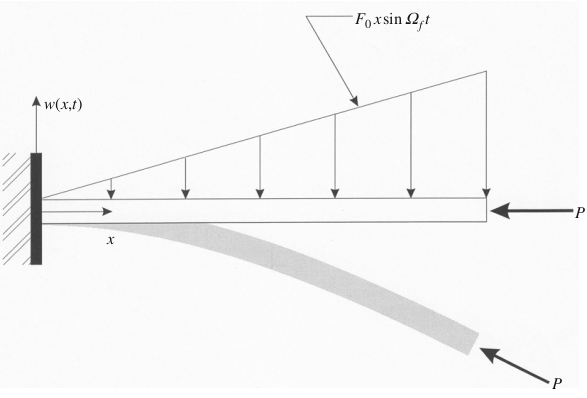
\includegraphics[height=8cm]{fig_2_2}
	\caption{Cantilever beam subjected to a tangential, follower compressive load, $P$ and a time-dependent distributed force, $F(x,t)$}
	\label{fig:forcing}
\end{figure}                   


\subsection{Non-dimensionalization of the equation} The equation \ref{eqn:cantilever-beam-forced} consists of the following physical variables
$$x, L, w, E, I, m, P, F, t, \Omega_f$$
Denoting dimension of mass by $\mathcal{M}$, dimension of length by $\mathcal{M}$ and dimension of time by $\mathcal{T}$, let us construct a time scale as 
$$\sqrt{\frac{mL^4}{EI}} \equiv \sqrt{\frac{\mathcal{ML}^{-1}\mathcal{L}^4}{(\mathcal{M}\mathcal{L}^{-1}\mathcal{T}^{-2})(\mathcal{L}^4)}} = \mathcal{T}$$
Let us non-dimensionalize the variables as

\begin{minipage}{0.5\textwidth}
	\begin{itemize}
		\item $\xi = \frac{x}{L} \equiv \frac{\mathcal{L}}{\mathcal{L}}$
		\item $\eta = \frac{w}{L} \equiv \frac{\mathcal{L}}{\mathcal{L}}$
		\item $\tau = \frac{t}{\sqrt{\frac{mL^4}{EI}}} \equiv \frac{\mathcal{T}}{\mathcal{T}}$
		\item $\mathcal{P} = \frac{PL^2}{EI} \equiv \frac{(\mathcal{M}\mathcal{L}\mathcal{T}^{-2})(\mathcal{L}^2)}{(\mathcal{M}\mathcal{L}^{-1}\mathcal{T}^{-2})(\mathcal{L}^4)}$
		\item $f = \frac{FL^3}{EI} \equiv \frac{(\mathcal{M}\mathcal{T}^{-2})(\mathcal{L}^3)}{(\mathcal{M}\mathcal{L}^{-1}\mathcal{T}^{-2})(\mathcal{L}^4)}$
		\item $\omega_f = \Omega_f\sqrt{\frac{mL^4}{EI}} \equiv \frac{\mathcal{T}}{\mathcal{T}^{-1}}$
	\end{itemize}
\end{minipage}

For the given problem, $F(x,t) = F_0 x \sin (\Omega_f t)$ and its non-dimensional counterpart is 
$$f = \frac{F_0 x \sin (\Omega_f t)~L^3}{EI} = \underbrace{\frac{F_0 L^4}{EI}}_{f_0}\underbrace{\frac{x}{L}}_\xi\sin (\frac{\omega_f}{\sqrt{\frac{mL^4}{EI}}} t) = f_0\xi \sin(\omega_f \tau)$$

Dividing both sides of equation \ref{eqn:cantilever-beam-forced} by $\frac{EI}{L^3}$, we get
\begin{align*}
L^3\pdv[4]{w}{x} + \frac{PL^3}{EI}\pdv[2]{w}{x} + \frac{mL^3}{EI}\pdv[2]{w}{t} &= \frac{F(x,t)L^3}{EI} \\
L^3\pdv[4]{(\eta L)}{(\xi L)} + \frac{PL^3}{EI}\pdv[2]{(\eta L)}{(\xi L)} + \frac{mL^3}{EI}\pdv[2]{(\eta L)}{\left(\sqrt{\frac{mL^4}{EI}}\tau\right) } &= \frac{F(x,t)L^3}{EI} \\
\implies \qquad \pdv[4]{\eta }{\xi} + \mathcal{P}\pdv[2]{\eta}{\xi} + \pdv[2]{\eta }{\tau} &= 0 \\
\implies \qquad \eta^{''''} + \mathcal{P} \eta^{''} + \ddot{\eta} &= f_0\xi \sin(\omega_f \tau) 
\end{align*}
where primes and dots indicate partial differentiation with respect to $\xi$ and $\tau$.

Substituting $\eta (\xi, \tau) \approx \eta_N (\xi, \tau) = \sum_{j=1}^N \phi_j(\xi)q_j(\tau)$ in the above equation, multiplying $\phi (\xi)$ on both sides and integrating from $\xi = 0$ to $\xi = 1$, we get
\begin{align*}
\sum_{j=1}^N\left( \int_0^1 \dv[4]{\phi_j (\xi)}{\xi}\phi_i (\xi) d\xi + \mathcal{P}\int_0^1 \dv[2]{\phi_j (\xi)}{\xi}\phi_i (\xi) d\xi \right) q_j (\tau) &\\
~+ \sum_{j=1}^N\left(\int_0^1 \phi_i(\xi) \phi_j(\xi) d\xi\right) \ddot{q}_j(\tau) &= \int_0^1 f_0\xi \sin(\omega_f \tau) d\xi \\
\sum_{j=1}^N \left(k_{ij} q_j (\tau) + \delta_{ij} \ddot{q}_j(\tau) \right) &= Q_i \sin(\omega_f \tau);~ i=1,2, \cdots, N \\
\implies~\sum_{j=1}^N \left(m_{ij} \ddot{q}_j(\tau) + k_{ij} q_j (\tau)\right) &= Q_i \sin(\omega_f \tau);~ i=1,2, \cdots, N
\end{align*}
where, 
\begin{itemize}
	\item $k_{ij} = \int_0^1 \dv[4]{\phi_j (\xi)}{\xi}\phi_i (\xi) d\xi + \mathcal{P}\int_0^1 \dv[2]{\phi_j (\xi)}{\xi}\phi_i (\xi) d\xi$
	\item $\int_0^1 \phi_i(\xi) \phi_j(\xi) d\xi = \delta_{ij}$
	\item $\int_0^1 \phi_i(\xi) \phi_j(\xi) d\xi = \delta_{ij}, Q_j = \int_0^1 f_0\xi d\xi$
\end{itemize}
We have the following matrix equation
\begin{align}
[I]\{\ddot{q}\} + [K]\{q\} &= \{Q\}\sin(\omega_f \tau) \label{eqn:reduced-matrix-eqn-forced}
\end{align} 
where $[I]$ is the unit matrix
\subsection{Decoupling the equation} As the matrix $[K]$ is asymmetric, we need to resort to biorthogonalization technique to decouple the eqn \ref{eqn:reduced-matrix-eqn-forced}.
Let us determine the eigenvalues, left and right eigenvectors of $[K]$. The right eigenvectors are determined as
\begin{align*}
[K][X] &= [X][\Lambda] 
\end{align*}
where the columns of $[X]$ are the right eigenvectors and $[\Lambda]$ is a diagonal matrix containing the eigenvalues.
The left eigenvectors of $[K]$ are the right eigenvectors of the tranpose of  $[K]$, that is, $[K]^T$
\begin{align*}
[K]^T[Y] &= [Y][\Lambda] \\
\implies [Y]^T[K] &= [\Lambda][Y]^T \quad \text{(tranposing both sides )}
\end{align*}
where the columns of $[Y]$ are the left eigenvectors of $[K]$ and $[\Lambda]$ is the diagonal matrix containing the eigenvalues.
The matrices are orthonormalized such that 
$$[Y]^T[X] = [I]$$
We can express $[K]$ as 
$$[K]=  [Y]^T[\Lambda][X]\quad \text{or } [Y]^T[K][X] = [\Lambda] $$
Introducing a transformation of the form $\{q\} = [X]\{y\}$ in the equation \ref{eqn:reduced-matrix-eqn-forced}, pre-multiplying both sides by $[Y]^T$, we have
\begin{align*}
[I][X]\{\ddot{y}\} + [K][X]\{y\} &= \{Q\}\sin(\omega_f \tau) \\
[Y]^T[X]\{\ddot{y}\} + [Y]^T[K][X]\{y\} &= [Y]^T\{Q\}\sin(\omega_f \tau) \\
\implies \{\ddot{y}\} + [\Lambda]\{y\} &= \{\Psi\}\sin(\omega_f \tau)
\end{align*}
The above equation now reduces to a set of ordinary differential equations or modal equations of the form
\begin{equation}
\ddot{y}_k + \Lambda_k y_k = \Psi_k \sin(\omega_f \tau), \quad k=1,2,\cdots, N \label{eqn:uncoupled-eqn-forced}
\end{equation}
The free response is given by the solution to its homogeneous form, that is,
\begin{equation}
\ddot{y}_k + \Lambda_k y_k = 0, \quad k=1,2,\cdots, N
\end{equation}
is given by $y_k = \alpha_k \cos(\Lambda_k^{1/2}\tau) + \beta_k \sin(\Lambda_k^{1/2}\tau)$ (assuming that $\Lambda_k$ is real) where $\alpha$ and $\beta_k$ are the constants of integration
For forced response, let us assume a solution of the form $y_k = C\sin(\omega_f \tau) + D \cos(\omega_f \tau)$ and put it into the equation \ref{eqn:uncoupled-eqn-forced}
\begin{align*}
-\omega_f^2(C\sin(\omega_f \tau) + D \cos(\omega_f \tau) + \Lambda_k (C\sin(\omega_f \tau) + D \cos(\omega_f \tau)) &= \Psi_k \sin(\omega_f \tau) \\
C(\Lambda_k - \omega_f^2) \sin(\omega_f \tau) + D(\Lambda_k - \omega_f^2) \cos(\omega_f \tau) &= \Psi_k \sin(\omega_f \tau) \\
\implies C = \frac{\Psi_k}{(\Lambda_k - \omega_f^2)}, &\phantom{=}~ D = 0
\end{align*}
Thus, the complete response to eqn \ref{eqn:uncoupled-eqn-forced} is 
$$y_k = \alpha_k \cos(\Lambda_k^{1/2}\tau) + \beta_k \sin(\Lambda_k^{1/2}\tau) + \frac{\Psi_k}{(\Lambda_k - \omega_f^2)}\sin(\omega_f \tau), \quad k=1,2,\cdots,N $$






%\paragraph{Free response} The equation \ref{eqn:matrix-equation} is solved to obtain the free response of the system for a given set of initial conditions.
%Multiply both sides of eqn \ref{eqn:matrix-equation} by $[M]^{-1}$ (assuming $[M]$ is invertible) to get
%\begin{align}
%\{\ddot{q}\} + [W]\{q\} &= \{0\}; \qquad [W] = [M]^{-1}[K] \label{eqn:reduced-matrix-eqn}
%\end{align}
%Let us introduce an oscillatory solution of the form 
%\begin{align*}
%\{q\} &= \{A\}e^{i\Omega t} 
%\end{align*}
%where $\{A\}$ is the column of unknown amplitudes and $\Omega$ the circular frequency
%\begin{align*}
%-\Omega^2\{A\}e^{i\Omega t} + [W]\{A\}e^{i\Omega t} &= \{0\} \\
%\implies \left( [W] - \Omega^2[I]\right) \{A\} &= \{0\}  \qquad [I] \text{ is the identity matrix} 
%\end{align*}
%For non-trivial solution, we must have the following characteristic equation
%$\det([W] - \Omega^2[I]) = 0$
%from which we can obtain $\Omega_i^2,~i=1,2,\cdots, N$ and also their corresponding eigenvectors $\{A\}_i$.
%
%To decouple the equation \ref{eqn:reduced-matrix-eqn}, we introduce the following transformation
%\begin{align}
%\{q\} &= [A]\{y\} \label{eqn:transformation}
%\end{align}
%where the modal matrix, $[A] = [\{A\}_1~\{A\}_2~\cdots~\{A\}_N]$ and $\{y\}$ contains the principal coordinates
%
%Suppose that the eigenvalues are real despite $[K]$ being asymmetric and linearly independent eigenvectors have been found,
%Substituting eqn \ref{eqn:transformation} in \ref{eqn:reduced-matrix-eqn} and pre-multiplying both sides by $[A]^{-1}$, we have
%\begin{align}
%\{\ddot{y}\} &= 
%\end{align}


%%%%%%%%%%%%% References
\begin{thebibliography}{99}
	\bibitem{paidoussis1993}
	Paidoussis, Michael P., Li, G. X. (1993), ``Pipes conveying fluid: A model dynamical problem'', \textit{Jour of Fluids and Structures} 7, 137-204
	
	\bibitem{paidoussis1974}
	Paidoussis, Michael P., Issid, N. T. (1974), ``Dynamic stability of pipes conveying fluid'', \textit{Jour of Sound and Vibration} 33 (3), 267-294
	
	\bibitem{paidoussis}
	Paidoussis, Michael P. (2014), \textit{Fluid-Structure Interactions: Slender Structures and Axial Flow Volume 1}, Academic Press, Oxford, UK
	
	\bibitem{meirovitch}
	Meirovitch, Leonard (2001), \textit{Fundamentals of Vibrations}, McGraw-Hill, Singapore
	
	\bibitem{gregory1966}
	Gregory, R. W., Paidoussis, Michael P. (1966), ``Unstable oscillation of tubular cantilevers conveying fluid I: Theory'', \textit{Proceedings of the Royal Society (London)} 293, 512-527
	
	\bibitem{scipy-documentation}
	Scientific Python documentation (2020), \url{https://docs.scipy.org/doc/scipy/reference/tutorial/integrate.html}
	
	\bibitem{python-control}
	\textit{Python Control Systems Library} (2020), \url{http://www.python-control.org}
	
	\bibitem{my-github}
	Avatar, G. R. Krishna Chand (2021), ``Python code for linear dynamics of a cantilevered pipe conveying fluid'', \url{https://github.com/kcavatar/cantilevered-pipe-conveying-fluid}
	
\end{thebibliography}

%%%%%%%%%%%%%%%%%%%%%% APPENDIX
\appendixpage

\appendix

\chapter{Derivation of cantilever beam modal functions}\label{app:cantilever-beam-modes}

Consider the following non-dimensional equation of a cantilever beam 
\begin{align}
  %\pdv[2]{\eta}{\tau} + \pdv[4]{\eta}{\xi} = 0 \\
  \qquad\qquad \ddot{\eta} + \eta'''' = 0 \label{app-eqn:cantilever-beam}
\end{align}
Introduce a solution of the form \cite{meirovitch}
$$\eta (\xi, \tau) = q (\tau) \phi (\xi)$$
On substituting the above expression into eqn \ref{app-eqn:cantilever-beam}, we have
\begin{align}
   \ddot{q}\phi + q\phi'' = 0 \notag \\
    -\frac{\ddot{q}}{q} = \frac{\phi''''}{\phi}  = k ~(\text{constant}) \label{app-eqn:2}
\end{align}
For harmonic solution, we must have $k = \omega^2$  and so
\begin{align}
 \phi'''' &= \omega^2 \phi  \notag  \\
 \implies ~\phi'''' - \omega^2 \phi &= 0 \label{app-eqn:3}
\end{align}
Takiing $\lambda^4 = \omega^2$, we have
\begin{align}
  \phi'''' - \lambda^4 \phi &= 0 \label{app-eqn:4}
\end{align}
The eqn \ref{app-eqn:4} accepts a solution of the form 
\begin{align}
  \phi(\xi) = A \cosh (\lambda \xi) + B \cos (\lambda \xi) + C\sinh(\lambda \xi) + D\sin(\lambda \xi) \label{app-eqn:5}
\end{align}
The boundary conditions for the cantilever beam are
\begin{align}
 \phi(\xi = 0) = \phi(\xi = 0) = \phi''(\xi = 1) = \phi''' (\xi = 0) = 0 \label{app-eqn:6}
\end{align}
Applying the first boundary condition (b.c.) given in eqn \ref{app-eqn:6} to eqn \ref{app-eqn:5}, we have
\begin{align}
       0 &= A + B \notag \\
       B &= - A \label{app-eqn:7}
\end{align}
Applying the second b.c. given in eqn \ref{app-eqn:6}, 
\begin{align}
  \phi(\xi) &= \lambda (A \sinh (\lambda \xi) - B \sin (\lambda \xi) + C\cosh(\lambda \xi) + D\cos(\lambda \xi))  \notag  \\
  \implies~ 0 &= \lambda (C + D) \notag \\
  \implies~ D &= -C \label{app-eqn:8}
\end{align}
Applying the third b.c., $\phi''(\xi = 1) = 0$, given in eqn \ref{app-eqn:6}, and using eqns \ref{app-eqn:7} and \ref{app-eqn:8}
\begin{align}
  \phi''(\xi) &=  \lambda^2 (A \cosh (\lambda \xi) - B \cos (\lambda \xi) + C\sinh(\lambda \xi) - D\sin(\lambda \xi))  \notag  \\
  \implies~~      0  &= \lambda^2 (A \cosh (\lambda) - B \cos (\lambda) + C\sinh(\lambda) - D\sin(\lambda))\notag \\
   \implies~~   0 &= A (\cosh (\lambda) + \cos (\lambda)) + C(\sinh(\lambda) + \sin(\lambda)) \notag  \\
   \implies ~~ \frac{C}{A} &= - \frac{(\cosh (\lambda) + \cos (\lambda)}{(\sinh(\lambda) + \sin(\lambda))} \label{app-eqn:9}
\end{align}
Applying the fourth b.c., $\phi'''(\xi = 1) = 0$, given in eqn \ref{app-eqn:6}, and using eqns \ref{app-eqn:7} and \ref{app-eqn:8}
\begin{align}
\phi'''(\xi) &=  \lambda^3 (A \sinh (\lambda \xi) + B \sin (\lambda \xi) + C\cosh(\lambda \xi) - D\cos(\lambda \xi))  \notag  \\
\implies~~      0  &= \lambda^3 (A \sinh (\lambda) + B \sin (\lambda) + C\cosh(\lambda) - D\cos(\lambda))\notag \\
\implies~~   0 &= A (\sinh (\lambda) - \sin (\lambda)) + C(\cosh(\lambda) + \cos(\lambda)) \notag  \\
\implies ~~ \frac{C}{A} &= - \frac{(\sinh (\lambda) - \sin (\lambda)}{(\cosh (\lambda) + \cos (\lambda))} \label{app-eqn:10}
\end{align}
From eqns \ref{app-eqn:9} and \ref{app-eqn:10},
\begin{align}
   \frac{(\cosh (\lambda) + \cos (\lambda)}{(\sinh(\lambda) + \sin(\lambda))} &= \frac{(\sinh (\lambda) - \sin (\lambda)}{(\cosh (\lambda) + \cos (\lambda))} \notag \\
   \implies~~ \cosh^2(\lambda) + \cos^2(\lambda) + 2 \cosh(\lambda)\cos(\lambda) &= \sinh^2(\lambda) - \sin^2(\lambda) \notag \\
   \implies~~\underbrace{\cosh^2(\lambda) - \sinh^2(\lambda)}_{1} + \underbrace{\cos^2(\lambda) + \sin^2(\lambda)}_{1} + 2 \cosh(\lambda)\cos(\lambda) &= 0 \notag \\
   \implies~~ 2 + 2 \cosh(\lambda)\cos(\lambda) &= 0  \notag \\
   \implies~~ 1 + \cosh(\lambda)\cos(\lambda) &= 0  \label{app-eqn:11} 
\end{align}
The transcendental equation \ref{app-eqn:11} is the characteristic equation of the cantilever beam. The roots of eqn \ref{app-eqn:11} gives the modal frequencies $\omega_r = \lambda_r^2$ satisfying 
\begin{align*}
 1 + \cosh(\lambda_r)\cos(\lambda_r) &= 0 \qquad r = 1, 2, \dots
\end{align*}
Using eqns \ref{app-eqn:7} and \ref{app-eqn:8}, we have the following expression for the $r^{\text{th}}$ modal function \ref{app-eqn:5}
\begin{align*}
\phi_r(\xi) &= A \bigg(\cosh (\lambda_r \xi) - \cos (\lambda_r \xi)\bigg) + C\bigg(\sinh(\lambda_r \xi) - \sin(\lambda_r \xi) \bigg) \qquad r = 1, 2, \dots \\
       &= A_r \bigg[\cosh (\lambda_r \xi) - \cos (\lambda_r \xi) + \frac{C_r}{A_r}\bigg(\sinh(\lambda_r \xi) - \sin(\lambda_r \xi) \bigg)\bigg] \qquad r = 1, 2, \dots
\end{align*}
We could use any one of eqns \ref{app-eqn:7} and \ref{app-eqn:8} to substitute for $\frac{C_r}{A_r}$. Picking $\frac{C_r}{A_r} = -\frac{(\sinh (\lambda_r) - \sin (\lambda_r)}{(\cosh (\lambda_r) + \cos (\lambda_r))} $, we have the $r^{\text{th}}$ modal function
\begin{align}
\phi_r(\xi) &= A_r \bigg[\cosh (\lambda_r \xi) - \cos (\lambda_r \xi) -\frac{(\sinh (\lambda_r) - \sin (\lambda_r))}{(\cosh (\lambda_r) + \cos (\lambda_r))}\bigg(\sinh(\lambda_r \xi) - \sin(\lambda_r \xi) \bigg)\bigg] \qquad r = 1, 2, \dots \label{app-bin:modal-function}
\end{align}
We normalize the above expression so that  $A_r$ is no longer arbitrary as
\begin{align*}
  \int_{0}^1 \phi_r^2 (\xi) ~d\xi = 1 \qquad r = 1, 2, \dots
\end{align*}
\paragraph{Orthogonality of modal functions} The normalized modal functions are orthonormal such that
\begin{align*}
       \int_{0}^1 \phi_r (\xi) \phi_s (\xi) ~d\xi = \delta_{rs} \qquad r, s = 1, 2, \dots
\end{align*}
where the Kronecker delta $\delta_{rs} = 1$ if $r = s$ and $\delta_{rs} = 0$ if $r \neq s$

\end{document}